\documentclass[a4paper]{book}
\usepackage{a4wide}
\usepackage{makeidx}
\usepackage{graphicx}
\usepackage{multicol}
\usepackage{float}
\usepackage{listings}
\usepackage{color}
\usepackage{textcomp}
\usepackage{alltt}
\usepackage{times}
\usepackage{ifpdf}
\ifpdf
\usepackage[pdftex,
            pagebackref=true,
            colorlinks=true,
            linkcolor=blue,
            unicode
           ]{hyperref}
\else
\usepackage[ps2pdf,
            pagebackref=true,
            colorlinks=true,
            linkcolor=blue,
            unicode
           ]{hyperref}
\usepackage{pspicture}
\fi
\usepackage[utf8]{inputenc}
\usepackage{doxygen}
\lstset{language=C++,inputencoding=utf8,basicstyle=\footnotesize,breaklines=true,breakatwhitespace=true,tabsize=8,numbers=left }
\makeindex
\setcounter{tocdepth}{3}
\renewcommand{\footrulewidth}{0.4pt}
\begin{document}
\hypersetup{pageanchor=false}
\begin{titlepage}
\vspace*{7cm}
\begin{center}
{\Large muTrade API 2.1 Python Interface }\\
\vspace*{1cm}
{\large Generated by Doxygen 1.6.1}\\
\vspace*{0.5cm}
{\small Wed May 6 16:48:25 2015}\\
\end{center}
\end{titlepage}
\clearemptydoublepage
\pagenumbering{roman}
\tableofcontents
\clearemptydoublepage
\pagenumbering{arabic}
\hypersetup{pageanchor=true}
\chapter{Namespace Index}
\section{Namespace List}
Here is a list of all documented namespaces with brief descriptions\-:\begin{DoxyCompactList}
\item\contentsline{section}{\hyperlink{namespacemuTradePyBase}{mu\-Trade\-Py\-Base} }{\pageref{namespacemuTradePyBase}}{}
\end{DoxyCompactList}

\chapter{Class Index}
\section{Class Hierarchy}
This inheritance list is sorted roughly, but not completely, alphabetically:\begin{DoxyCompactList}
\item \contentsline{section}{muTradePyBase::CustomStrategy}{\pageref{classmuTradePyBase_1_1CustomStrategy}}{}
\begin{DoxyCompactList}
\item \contentsline{section}{sampleStrategy::sample}{\pageref{classsampleStrategy_1_1sample}}{}
\end{DoxyCompactList}
\end{DoxyCompactList}

\chapter{Class Index}
\section{Class List}
Here are the classes, structs, unions and interfaces with brief descriptions\-:\begin{DoxyCompactList}
\item\contentsline{section}{\hyperlink{struct_a_p_i2_1_1_duplicate_key_exception}{A\-P\-I2\-::\-Duplicate\-Key\-Exception} \\*The \hyperlink{struct_a_p_i2_1_1_duplicate_key_exception}{Duplicate\-Key\-Exception} struct }{\pageref{struct_a_p_i2_1_1_duplicate_key_exception}}{}
\item\contentsline{section}{\hyperlink{class_a_p_i2_1_1_c_o_m_m_o_n_1_1_instrument}{A\-P\-I2\-::\-C\-O\-M\-M\-O\-N\-::\-Instrument} \\*Provides all the information about Market \hyperlink{class_a_p_i2_1_1_c_o_m_m_o_n_1_1_instrument}{Instrument} }{\pageref{class_a_p_i2_1_1_c_o_m_m_o_n_1_1_instrument}}{}
\item\contentsline{section}{\hyperlink{struct_a_p_i2_1_1_c_o_m_m_o_n_1_1_instrument_position}{A\-P\-I2\-::\-C\-O\-M\-M\-O\-N\-::\-Instrument\-Position} \\*The \hyperlink{struct_a_p_i2_1_1_c_o_m_m_o_n_1_1_instrument_position}{Instrument\-Position} struct Provides the basic information like Open Qty, Open\-Side, Traded Quantity in Buy/\-Sell Side, \par
 Average traded Price in Buy/\-Sell Side, Booked and Mark-\/\-To-\/\-Market Profit and loss }{\pageref{struct_a_p_i2_1_1_c_o_m_m_o_n_1_1_instrument_position}}{}
\item\contentsline{section}{\hyperlink{struct_a_p_i2_1_1_market_data_subscription_failed_exception}{A\-P\-I2\-::\-Market\-Data\-Subscription\-Failed\-Exception} \\*The \hyperlink{struct_a_p_i2_1_1_market_data_subscription_failed_exception}{Market\-Data\-Subscription\-Failed\-Exception} struct }{\pageref{struct_a_p_i2_1_1_market_data_subscription_failed_exception}}{}
\item\contentsline{section}{\hyperlink{class_a_p_i2_1_1_c_o_m_m_o_n_1_1_market_data_wrapper}{A\-P\-I2\-::\-C\-O\-M\-M\-O\-N\-::\-Market\-Data\-Wrapper} \\*Will contain the Snapshot/\-T\-B\-T Market Data }{\pageref{class_a_p_i2_1_1_c_o_m_m_o_n_1_1_market_data_wrapper}}{}
\item\contentsline{section}{\hyperlink{class_a_p_i2_1_1_c_o_m_m_o_n_1_1_market_depth_wrapper}{A\-P\-I2\-::\-C\-O\-M\-M\-O\-N\-::\-Market\-Depth\-Wrapper} \\*Will store Bid Ask Price at particular level }{\pageref{class_a_p_i2_1_1_c_o_m_m_o_n_1_1_market_depth_wrapper}}{}
\item\contentsline{section}{\hyperlink{class_a_p_i2_1_1_c_o_m_m_o_n_1_1_mkt_data}{A\-P\-I2\-::\-C\-O\-M\-M\-O\-N\-::\-Mkt\-Data} \\*The \hyperlink{class_a_p_i2_1_1_c_o_m_m_o_n_1_1_mkt_data}{Mkt\-Data} class, The wrapper class for getting Market Feed for both Snapshot and Tick-\/\-By-\/\-Tick }{\pageref{class_a_p_i2_1_1_c_o_m_m_o_n_1_1_mkt_data}}{}
\item\contentsline{section}{\hyperlink{class_a_p_i2_1_1_order_confirmation}{A\-P\-I2\-::\-Order\-Confirmation} \\*Exchange Order Confirmation Message data }{\pageref{class_a_p_i2_1_1_order_confirmation}}{}
\item\contentsline{section}{\hyperlink{class_a_p_i2_1_1_s_g_context}{A\-P\-I2\-::\-S\-G\-Context} \\*The main class to be inherited for creating a new Strategy }{\pageref{class_a_p_i2_1_1_s_g_context}}{}
\item\contentsline{section}{\hyperlink{class_a_p_i2_1_1_single_order}{A\-P\-I2\-::\-Single\-Order} \\*The \hyperlink{class_a_p_i2_1_1_single_order}{Single\-Order} class. This wrapper is used for sending Single Leg Orders. Usage\-: Create an object for This using \hyperlink{class_a_p_i2_1_1_s_g_context_ab141f05e2a0d8a51fdadc57bf53d2cd8}{A\-P\-I2\-::\-S\-G\-Context\-::create\-New\-Order} }{\pageref{class_a_p_i2_1_1_single_order}}{}
\item\contentsline{section}{\hyperlink{class_a_p_i2_1_1_strategy_parameters}{A\-P\-I2\-::\-Strategy\-Parameters} \\*Basic Strategy Parameters, Strategy\-Id and Client\-Id.\par
 Stratgy Parameters are provided by \hyperlink{class_a_p_i2_1_1_strategy_parameters_a6a7c4d4c3e6cae23741c87732e89689a}{Strategy\-Parameters\-::get\-Info()} }{\pageref{class_a_p_i2_1_1_strategy_parameters}}{}
\item\contentsline{section}{\hyperlink{struct_a_p_i2_1_1_symbol_static_data}{A\-P\-I2\-::\-Symbol\-Static\-Data} \\*The A\-P\-I\-\_\-\-Symbol\-Static\-Data struct }{\pageref{struct_a_p_i2_1_1_symbol_static_data}}{}
\item\contentsline{section}{\hyperlink{struct_a_p_i2_1_1_unknown_type_exception}{A\-P\-I2\-::\-Unknown\-Type\-Exception} \\*The \hyperlink{struct_a_p_i2_1_1_unknown_type_exception}{Unknown\-Type\-Exception} struct }{\pageref{struct_a_p_i2_1_1_unknown_type_exception}}{}
\item\contentsline{section}{\hyperlink{class_a_p_i2_1_1_user_params}{A\-P\-I2\-::\-User\-Params} \\*The A\-P\-I2\-\_\-\-User\-Params class }{\pageref{class_a_p_i2_1_1_user_params}}{}
\end{DoxyCompactList}

\chapter{File Index}
\section{File List}
Here is a list of all files with brief descriptions:\begin{DoxyCompactList}
\item\contentsline{section}{\hyperlink{muTradePyBase_8py}{muTradePyBase.py} }{\pageref{muTradePyBase_8py}}{}
\item\contentsline{section}{\hyperlink{README_8md}{README.md} }{\pageref{README_8md}}{}
\item\contentsline{section}{\hyperlink{sampleStrategy_8py}{sampleStrategy.py} }{\pageref{sampleStrategy_8py}}{}
\end{DoxyCompactList}

\chapter{Namespace Documentation}
\hypertarget{namespacemuTradePyBase}{\section{mu\-Trade\-Py\-Base Namespace Reference}
\label{namespacemuTradePyBase}\index{mu\-Trade\-Py\-Base@{mu\-Trade\-Py\-Base}}
}
\subsection*{Classes}
\begin{DoxyCompactItemize}
\item 
class \hyperlink{classmuTradePyBase_1_1CustomStrategy}{Custom\-Strategy}
\end{DoxyCompactItemize}


\subsection{Detailed Description}
\begin{DoxyVerb}@package pyApi
\end{DoxyVerb}
 
\hypertarget{namespacesampleStrategy}{
\section{sampleStrategy Namespace Reference}
\label{namespacesampleStrategy}\index{sampleStrategy@{sampleStrategy}}
}
\subsection*{Classes}
\begin{DoxyCompactItemize}
\item 
class \hyperlink{classsampleStrategy_1_1sample}{sample}
\end{DoxyCompactItemize}

\chapter{Class Documentation}
\hypertarget{classmuTradePyBase_1_1CustomStrategy}{
\section{muTradePyBase::CustomStrategy Class Reference}
\label{classmuTradePyBase_1_1CustomStrategy}\index{muTradePyBase::CustomStrategy@{muTradePyBase::CustomStrategy}}
}
Inheritance diagram for muTradePyBase::CustomStrategy::\begin{figure}[H]
\begin{center}
\leavevmode
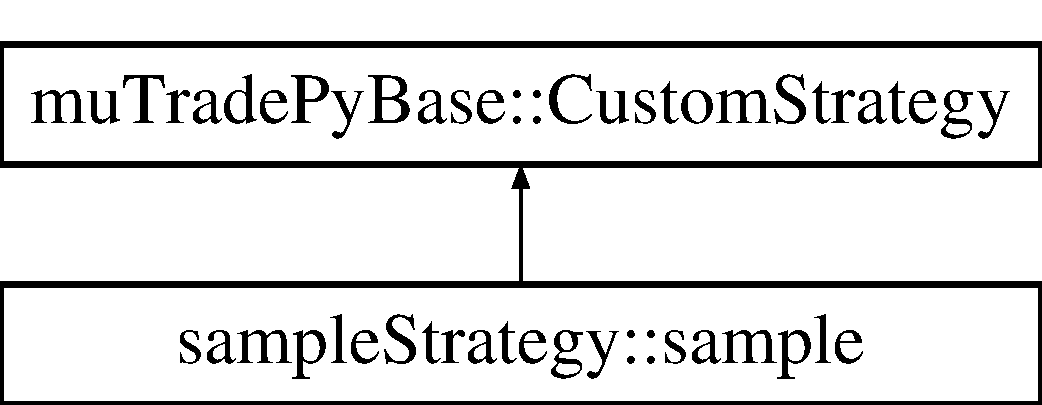
\includegraphics[height=2cm]{classmuTradePyBase_1_1CustomStrategy}
\end{center}
\end{figure}
\subsection*{Public Member Functions}
\begin{DoxyCompactItemize}
\item 
def \hyperlink{classmuTradePyBase_1_1CustomStrategy_ac6fcdf08165af5413c9883bf68dcd23b}{\_\-\_\-init\_\-\_\-}
\item 
def \hyperlink{classmuTradePyBase_1_1CustomStrategy_a8accc7202088d5163a9bffa940961713}{onInitEvent}
\begin{DoxyCompactList}\small\item\em Strategy's first event. \item\end{DoxyCompactList}\item 
def \hyperlink{classmuTradePyBase_1_1CustomStrategy_af8fb22d6864e7c61a61f94cf963746e5}{onCMDModifyStrategy}
\begin{DoxyCompactList}\small\item\em no \item\end{DoxyCompactList}\item 
def \hyperlink{classmuTradePyBase_1_1CustomStrategy_aeb2e0e2196645380512c59f9752efb5e}{onCMDTerminateStartegy}
\begin{DoxyCompactList}\small\item\em no \item\end{DoxyCompactList}\item 
def \hyperlink{classmuTradePyBase_1_1CustomStrategy_a8b35516aaa2a7f1940ad86191e022b8e}{onCMDTerminateSqOffStrategy}
\begin{DoxyCompactList}\small\item\em no \item\end{DoxyCompactList}\item 
def \hyperlink{classmuTradePyBase_1_1CustomStrategy_a30611f9dbe54a60219fcb95605004eaa}{onDefaultEvent}
\begin{DoxyCompactList}\small\item\em Default periodic event. \item\end{DoxyCompactList}\item 
def \hyperlink{classmuTradePyBase_1_1CustomStrategy_aea61c58829beb5f5e4bfa3355da9a23b}{onMarketDataEvent}
\begin{DoxyCompactList}\small\item\em Event when new market data is received. \item\end{DoxyCompactList}\item 
def \hyperlink{classmuTradePyBase_1_1CustomStrategy_aa94a2228807baeaab027108dc663675e}{onOhlcTimeOutEvent}
\item 
def \hyperlink{classmuTradePyBase_1_1CustomStrategy_a2d99ec0bbe867655ed7f9373812d7a56}{onConfirmed}
\begin{DoxyCompactList}\small\item\em On confirmation of order with orderid specified in it's argument. \item\end{DoxyCompactList}\item 
def \hyperlink{classmuTradePyBase_1_1CustomStrategy_a85a80a9afefdf345a46c520fad9b5138}{onReplaced}
\begin{DoxyCompactList}\small\item\em When the order with unique id : OrderId gets successfully replaced. \item\end{DoxyCompactList}\item 
def \hyperlink{classmuTradePyBase_1_1CustomStrategy_a2e18cb62689e42982bc46836f5fa156b}{onReplaceRejected}
\begin{DoxyCompactList}\small\item\em When request to replace order with id : OrderId is rejected due to reason specified by ErrorCode. \item\end{DoxyCompactList}\item 
def \hyperlink{classmuTradePyBase_1_1CustomStrategy_ac0dc077ece6c64c2a61ee3b9f511c680}{onCancelRejected}
\begin{DoxyCompactList}\small\item\em When the request to cancel an order is rejected. \item\end{DoxyCompactList}\item 
def \hyperlink{classmuTradePyBase_1_1CustomStrategy_ad17943f78d2a1a38716e94067eba0804}{onCanceled}
\begin{DoxyCompactList}\small\item\em When order with id : OrderId gets cancelled. \item\end{DoxyCompactList}\item 
def \hyperlink{classmuTradePyBase_1_1CustomStrategy_a5274ec9bdcddf755f17f2fc0817e4e19}{onNewRejected}
\begin{DoxyCompactList}\small\item\em when new placed order is rejected by the market \item\end{DoxyCompactList}\item 
def \hyperlink{classmuTradePyBase_1_1CustomStrategy_a409e9147a6d8d52dc2d3ad04544e31f3}{onIOCCanceled}
\begin{DoxyCompactList}\small\item\em When the some quantity of IOC order with id : OrderId was cancelled. \item\end{DoxyCompactList}\item 
def \hyperlink{classmuTradePyBase_1_1CustomStrategy_afade8f1587aab216a8aa6a7f0be1300f}{onFilled}
\begin{DoxyCompactList}\small\item\em When the order with id : OrderId was completely filled. \item\end{DoxyCompactList}\item 
def \hyperlink{classmuTradePyBase_1_1CustomStrategy_a5d2894514fc731a0298c2139435dbd20}{onPartialFill}
\begin{DoxyCompactList}\small\item\em When the order with id : OrderId was partially filled. \item\end{DoxyCompactList}\item 
def \hyperlink{classmuTradePyBase_1_1CustomStrategy_ab15e441859c93390410973beb565872a}{onMarketToLimit}
\begin{DoxyCompactList}\small\item\em order converted from market to limit \item\end{DoxyCompactList}\item 
def \hyperlink{classmuTradePyBase_1_1CustomStrategy_a40cb69958575c0a0a7e435d3ac0fe9f9}{onFrozen}
\begin{DoxyCompactList}\small\item\em when the order with id : OrderId gets frozen in the exchange \item\end{DoxyCompactList}\item 
def \hyperlink{classmuTradePyBase_1_1CustomStrategy_add6aa61bb18c2c3a4de459865fe83f62}{onTimerEvent}
\begin{DoxyCompactList}\small\item\em occurs after a periodic time interval as asked by the user \item\end{DoxyCompactList}\item 
def \hyperlink{classmuTradePyBase_1_1CustomStrategy_a71716af3dce670bfe2ec9a1d8a73afc3}{createInstrument}
\begin{DoxyCompactList}\small\item\em createNewInstrument To add a new Instrument in the strategy. \item\end{DoxyCompactList}\item 
def \hyperlink{classmuTradePyBase_1_1CustomStrategy_ab198cb371a98954673637288d3ab07c8}{createInstrumentFromSymbolFormat}
\begin{DoxyCompactList}\small\item\em createNewInstrument To add a new Instrument in the strategy. \item\end{DoxyCompactList}\item 
def \hyperlink{classmuTradePyBase_1_1CustomStrategy_ade3e0161fb897eed61c2ac3e1823ff8f}{reqPlaceNewOrder}
\begin{DoxyCompactList}\small\item\em places a new single order \item\end{DoxyCompactList}\item 
def \hyperlink{classmuTradePyBase_1_1CustomStrategy_aa6cbf9a067fcc64004f847d80913621c}{reqPlaceReplaceNewOrder}
\begin{DoxyCompactList}\small\item\em replaces an existing order with id : orderId by a new single order \item\end{DoxyCompactList}\item 
def \hyperlink{classmuTradePyBase_1_1CustomStrategy_a960f1c0ee467c21a732e1ae080b39dcb}{reqPlaceCancelOrder}
\begin{DoxyCompactList}\small\item\em cancels an existing single order with id : orderId \item\end{DoxyCompactList}\item 
def \hyperlink{classmuTradePyBase_1_1CustomStrategy_a67ba152e8e50acf69bc02ca08088bb0a}{reqStartAlgo}
\begin{DoxyCompactList}\small\item\em function call to Start the Strategy listening to OHLC update events \item\end{DoxyCompactList}\item 
def \hyperlink{classmuTradePyBase_1_1CustomStrategy_a25d6d4941b75233ee3c126c8ff9def54}{reqUpdateMarketData}
\begin{DoxyCompactList}\small\item\em reqUpdateMarketData To manually update Market Feed for all registered Instruments. \item\end{DoxyCompactList}\item 
def \hyperlink{classmuTradePyBase_1_1CustomStrategy_a45cf7b8c54ce0ac8a226c3006ae20901}{reqRegisterTimerEvent}
\begin{DoxyCompactList}\small\item\em To request for a Timer-\/Based event, The event to be called back in time duration passed as argument in microseconds. \item\end{DoxyCompactList}\item 
def \hyperlink{classmuTradePyBase_1_1CustomStrategy_a6ebd2277cb90f65608bd4d636087b61e}{reqTerminateStrategy}
\begin{DoxyCompactList}\small\item\em reqTerminateStrategy Called to Terminate Strategy. \item\end{DoxyCompactList}\item 
def \hyperlink{classmuTradePyBase_1_1CustomStrategy_aead1310f3a4aa6c69d792ed18669bec1}{reqTerminateSqOffStrategy}
\begin{DoxyCompactList}\small\item\em Called to Terminate strategy and Square-\/Off all Positions. \item\end{DoxyCompactList}\item 
def \hyperlink{classmuTradePyBase_1_1CustomStrategy_a5315fa269b26a64625c3a79362e357e1}{reqQryPrice}
\item 
def \hyperlink{classmuTradePyBase_1_1CustomStrategy_ad6a87ecd9032561036aa40f83ed4c34f}{reqQryQty}
\item 
def \hyperlink{classmuTradePyBase_1_1CustomStrategy_a652f9a24a6b95f2f960555e5593c1fee}{reqQryLastTradePrice}
\item 
def \hyperlink{classmuTradePyBase_1_1CustomStrategy_a0a48ea343fcdffbf9bb24bcb0384af1d}{reqQryLastTradeQty}
\item 
def \hyperlink{classmuTradePyBase_1_1CustomStrategy_a72c9d6257adaa1e0a568e09f0df0ef15}{reqQryOpenPrice}
\item 
def \hyperlink{classmuTradePyBase_1_1CustomStrategy_aa66a4eb7129af05c92f0beaf335dfcd3}{reqQryHighPrice}
\item 
def \hyperlink{classmuTradePyBase_1_1CustomStrategy_aaa79b2efd9d3edba03a3eccff9e59c18}{reqQryLowPrice}
\item 
def \hyperlink{classmuTradePyBase_1_1CustomStrategy_ad402881274c2432ec5018c2e3da3c6cf}{reqQryClosePrice}
\item 
def \hyperlink{classmuTradePyBase_1_1CustomStrategy_a45942a08cd5fd7cd63ca6873786e2249}{reqQryVolume}
\item 
def \hyperlink{classmuTradePyBase_1_1CustomStrategy_a7cc21237ff1f78abaa29a1c87adc8f7c}{reqQryQuoteLastUpdateTime}
\item 
def \hyperlink{classmuTradePyBase_1_1CustomStrategy_a3828d43f41c88b74b14b920f29f96f9b}{reqQryInstrumentId}
\item 
def \hyperlink{classmuTradePyBase_1_1CustomStrategy_a58823e909645a91e0c35d8a71cc947e5}{reqQryLastQuotedPrice}
\item 
def \hyperlink{classmuTradePyBase_1_1CustomStrategy_a44a5e9d557e3de1f6cc1ba7f1b192e40}{reqQryOpenQty}
\item 
def \hyperlink{classmuTradePyBase_1_1CustomStrategy_a4f5ff1338b2dab2bd1fc6a6262eda68b}{reqQryTradedQty}
\item 
def \hyperlink{classmuTradePyBase_1_1CustomStrategy_afa2494957cf0c4cc62ae833c6f293654}{reqQryOpenSide}
\item 
def \hyperlink{classmuTradePyBase_1_1CustomStrategy_a833fe1cfaf064a995fd4caa2cdc32683}{reqQryBookedPnl}
\item 
def \hyperlink{classmuTradePyBase_1_1CustomStrategy_a72d97c769d9d74c968e20ef5208b86e1}{reqQryMtmPnl}
\item 
def \hyperlink{classmuTradePyBase_1_1CustomStrategy_a831e1208c1c70bd5a6d461156aa9a77a}{reqQryAvgPrice}
\item 
def \hyperlink{classmuTradePyBase_1_1CustomStrategy_a58d72b142c0336af5b6e569f3ed500c4}{reqQryPendingQty}
\item 
def \hyperlink{classmuTradePyBase_1_1CustomStrategy_aaa13aee1b0102ed8d6d5c78d18bed8cc}{reqQryClientId}
\item 
def \hyperlink{classmuTradePyBase_1_1CustomStrategy_ab2bb976f03464a96a1eaad71384988c8}{reqQryNetBookedPL}
\item 
def \hyperlink{classmuTradePyBase_1_1CustomStrategy_af22277e5d655d83298baff704eb15c20}{reqQryNetMarkToMarkPL}
\item 
def \hyperlink{classmuTradePyBase_1_1CustomStrategy_affe1610052e184d5501345f1a3f14169}{reqQrySymbolId}
\item 
def \hyperlink{classmuTradePyBase_1_1CustomStrategy_a1bfe7ef1cd4ad2b136eb2e7bb97005a5}{reqQryInstrumentList}
\begin{DoxyCompactList}\small\item\em function not available yet \item\end{DoxyCompactList}\item 
def \hyperlink{classmuTradePyBase_1_1CustomStrategy_a4f86b387e2a4566bc34e49a6eed18683}{reqQryAllInstruments}
\begin{DoxyCompactList}\small\item\em function not available yet \item\end{DoxyCompactList}\item 
def \hyperlink{classmuTradePyBase_1_1CustomStrategy_a20cce64603fa41524a94e2c28231bb0d}{reqQryExchangeOrderId}
\item 
def \hyperlink{classmuTradePyBase_1_1CustomStrategy_aa1306213f1bd45974a0fdd370be58d22}{reqAddLogMessage}
\begin{DoxyCompactList}\small\item\em can add messages to logs \item\end{DoxyCompactList}\item 
def \hyperlink{classmuTradePyBase_1_1CustomStrategy_a15a75b52429194a1656ae5327df1d20e}{reqFlushLogMessage}
\begin{DoxyCompactList}\small\item\em flushes messages into a file \item\end{DoxyCompactList}\item 
def \hyperlink{classmuTradePyBase_1_1CustomStrategy_a17c1786aa8fe23b8edb06dd064a2ff11}{reqQryStrategyID}
\item 
def \hyperlink{classmuTradePyBase_1_1CustomStrategy_a1b353f46dffc755667c896b669a638fa}{reqQryOrderPendingQty}
\item 
def \hyperlink{classmuTradePyBase_1_1CustomStrategy_a5a88d3465201abc5a438f8a3cbd72149}{reqQryInstrumentPendingQty}
\item 
def \hyperlink{classmuTradePyBase_1_1CustomStrategy_a498436149088a84055d2d3793775956a}{reqQryClientOrderID}
\item 
def \hyperlink{classmuTradePyBase_1_1CustomStrategy_a0127eda99cf09acb990a26ccc63ac617}{reqQryOrderStatus}
\item 
def \hyperlink{classmuTradePyBase_1_1CustomStrategy_aaed973e7d7ddba726cde0eccd20cca27}{getMarketDataEventRequired}
\item 
def \hyperlink{classmuTradePyBase_1_1CustomStrategy_a67150cfa4a93fd0e33cfdb515264985c}{getOHLCDataEventRequired}
\end{DoxyCompactItemize}
\subsection*{Public Attributes}
\begin{DoxyCompactItemize}
\item 
\hyperlink{classmuTradePyBase_1_1CustomStrategy_aa800d9ce36ac2a140b0722db94ccdab9}{tokenId}
\item 
\hyperlink{classmuTradePyBase_1_1CustomStrategy_a6cd3aa3febbc8ad76120b43a7663301f}{f}
\end{DoxyCompactItemize}


\subsection{Member Function Documentation}
\hypertarget{classmuTradePyBase_1_1CustomStrategy_ac6fcdf08165af5413c9883bf68dcd23b}{
\index{muTradePyBase::CustomStrategy@{muTradePyBase::CustomStrategy}!\_\-\_\-init\_\-\_\-@{\_\-\_\-init\_\-\_\-}}
\index{\_\-\_\-init\_\-\_\-@{\_\-\_\-init\_\-\_\-}!muTradePyBase::CustomStrategy@{muTradePyBase::CustomStrategy}}
\subsubsection[{\_\-\_\-init\_\-\_\-}]{\setlength{\rightskip}{0pt plus 5cm}def muTradePyBase::CustomStrategy::\_\-\_\-init\_\-\_\- ( {\em self}, \/   {\em tokenId})}}
\label{classmuTradePyBase_1_1CustomStrategy_ac6fcdf08165af5413c9883bf68dcd23b}
\begin{DoxyVerb}The constructor\end{DoxyVerb}
 

Reimplemented in \hyperlink{classsampleStrategy_1_1sample_a9181fa2dc3d56ebe267718817dbc6941}{sampleStrategy::sample}.\hypertarget{classmuTradePyBase_1_1CustomStrategy_a71716af3dce670bfe2ec9a1d8a73afc3}{
\index{muTradePyBase::CustomStrategy@{muTradePyBase::CustomStrategy}!createInstrument@{createInstrument}}
\index{createInstrument@{createInstrument}!muTradePyBase::CustomStrategy@{muTradePyBase::CustomStrategy}}
\subsubsection[{createInstrument}]{\setlength{\rightskip}{0pt plus 5cm}def muTradePyBase::CustomStrategy::createInstrument ( {\em self}, \/   {\em InstrumentId}, \/   {\em RegisterMktData}, \/   {\em UseSnapshot}, \/   {\em UseOHCL})}}
\label{classmuTradePyBase_1_1CustomStrategy_a71716af3dce670bfe2ec9a1d8a73afc3}


createNewInstrument To add a new Instrument in the strategy. The Pointer to the added Instrument is set in instrument passed as reference 
\begin{DoxyParams}{Parameters}
\item[{\em symbolId}]System Unique ID for the Instrument as API2::DATA\_\-TYPES::SYMBOL\_\-ID \item[{\em regMktData}]set True to register for Market Data for the Instrument \item[{\em useSnapShot}]Set True if Snapshot Feed is to be used and False to use TBT-\/Feed \item[{\em useOhlc}]Set True if OHLC Heed is also required \end{DoxyParams}

\begin{DoxyExceptions}{Exceptions}
\item[{\em MarketDataSubscriptionFailedException}]\end{DoxyExceptions}
\begin{DoxyReturn}{Returns}
COMMON::Instrument Pointer 
\end{DoxyReturn}
\hypertarget{classmuTradePyBase_1_1CustomStrategy_ab198cb371a98954673637288d3ab07c8}{
\index{muTradePyBase::CustomStrategy@{muTradePyBase::CustomStrategy}!createInstrumentFromSymbolFormat@{createInstrumentFromSymbolFormat}}
\index{createInstrumentFromSymbolFormat@{createInstrumentFromSymbolFormat}!muTradePyBase::CustomStrategy@{muTradePyBase::CustomStrategy}}
\subsubsection[{createInstrumentFromSymbolFormat}]{\setlength{\rightskip}{0pt plus 5cm}def muTradePyBase::CustomStrategy::createInstrumentFromSymbolFormat ( {\em self}, \/   {\em InstrumentId}, \/   {\em RegisterMktData}, \/   {\em UseSnapshot}, \/   {\em UseOHCL})}}
\label{classmuTradePyBase_1_1CustomStrategy_ab198cb371a98954673637288d3ab07c8}


createNewInstrument To add a new Instrument in the strategy. The Pointer to the added Instrument is set in instrument passed as reference 
\begin{DoxyParams}{Parameters}
\item[{\em instrumentName}]Instrument Name Format: \mbox{[}ExchangeName\mbox{]} \mbox{[}Symbol\mbox{]} \mbox{[}Expiry(YYYYMMDD)\mbox{]} \mbox{[}StrikePrice\mbox{]} \mbox{[}C/P(For Call/Put)\mbox{]} Example: Cash Segment: NSE RELIANCE Futures Segment: NSE RELIANCE 20140828 Options Segment: NSE RELIANCE 20140828 980.00 C \item[{\em regMktData}]set True to register for Market Data for the Instrument \item[{\em useSnapShot}]Set True if Snapshot Feed is to be used and False to use TBT-\/Feed \item[{\em useOhlc}]Set True if OHLC Heed is also required \end{DoxyParams}
\begin{DoxyReturn}{Returns}
long Instrument 
\end{DoxyReturn}

\begin{DoxyExceptions}{Exceptions}
\item[{\em MarketDataSubscriptionFailedException}]\end{DoxyExceptions}
\hypertarget{classmuTradePyBase_1_1CustomStrategy_aaed973e7d7ddba726cde0eccd20cca27}{
\index{muTradePyBase::CustomStrategy@{muTradePyBase::CustomStrategy}!getMarketDataEventRequired@{getMarketDataEventRequired}}
\index{getMarketDataEventRequired@{getMarketDataEventRequired}!muTradePyBase::CustomStrategy@{muTradePyBase::CustomStrategy}}
\subsubsection[{getMarketDataEventRequired}]{\setlength{\rightskip}{0pt plus 5cm}def muTradePyBase::CustomStrategy::getMarketDataEventRequired ( {\em self})}}
\label{classmuTradePyBase_1_1CustomStrategy_aaed973e7d7ddba726cde0eccd20cca27}
\begin{DoxyReturn}{Returns}
market data event flag 
\end{DoxyReturn}
\hypertarget{classmuTradePyBase_1_1CustomStrategy_a67150cfa4a93fd0e33cfdb515264985c}{
\index{muTradePyBase::CustomStrategy@{muTradePyBase::CustomStrategy}!getOHLCDataEventRequired@{getOHLCDataEventRequired}}
\index{getOHLCDataEventRequired@{getOHLCDataEventRequired}!muTradePyBase::CustomStrategy@{muTradePyBase::CustomStrategy}}
\subsubsection[{getOHLCDataEventRequired}]{\setlength{\rightskip}{0pt plus 5cm}def muTradePyBase::CustomStrategy::getOHLCDataEventRequired ( {\em self})}}
\label{classmuTradePyBase_1_1CustomStrategy_a67150cfa4a93fd0e33cfdb515264985c}
\begin{DoxyReturn}{Returns}
OHLC flag 
\end{DoxyReturn}
\hypertarget{classmuTradePyBase_1_1CustomStrategy_ad17943f78d2a1a38716e94067eba0804}{
\index{muTradePyBase::CustomStrategy@{muTradePyBase::CustomStrategy}!onCanceled@{onCanceled}}
\index{onCanceled@{onCanceled}!muTradePyBase::CustomStrategy@{muTradePyBase::CustomStrategy}}
\subsubsection[{onCanceled}]{\setlength{\rightskip}{0pt plus 5cm}def muTradePyBase::CustomStrategy::onCanceled ( {\em self}, \/   {\em OrderId})}}
\label{classmuTradePyBase_1_1CustomStrategy_ad17943f78d2a1a38716e94067eba0804}


When order with id : OrderId gets cancelled. 
\begin{DoxyParams}{Parameters}
\item[{\em OrderId}]unique id of the order that was cancelled \end{DoxyParams}
\hypertarget{classmuTradePyBase_1_1CustomStrategy_ac0dc077ece6c64c2a61ee3b9f511c680}{
\index{muTradePyBase::CustomStrategy@{muTradePyBase::CustomStrategy}!onCancelRejected@{onCancelRejected}}
\index{onCancelRejected@{onCancelRejected}!muTradePyBase::CustomStrategy@{muTradePyBase::CustomStrategy}}
\subsubsection[{onCancelRejected}]{\setlength{\rightskip}{0pt plus 5cm}def muTradePyBase::CustomStrategy::onCancelRejected ( {\em self}, \/   {\em OrderId}, \/   {\em ErrorCode})}}
\label{classmuTradePyBase_1_1CustomStrategy_ac0dc077ece6c64c2a61ee3b9f511c680}


When the request to cancel an order is rejected. 
\begin{DoxyParams}{Parameters}
\item[{\em OrderId}]unique id of the order to be cancelled \item[{\em ErrorCode}]reason for rejection \end{DoxyParams}
\hypertarget{classmuTradePyBase_1_1CustomStrategy_af8fb22d6864e7c61a61f94cf963746e5}{
\index{muTradePyBase::CustomStrategy@{muTradePyBase::CustomStrategy}!onCMDModifyStrategy@{onCMDModifyStrategy}}
\index{onCMDModifyStrategy@{onCMDModifyStrategy}!muTradePyBase::CustomStrategy@{muTradePyBase::CustomStrategy}}
\subsubsection[{onCMDModifyStrategy}]{\setlength{\rightskip}{0pt plus 5cm}def muTradePyBase::CustomStrategy::onCMDModifyStrategy ( {\em self})}}
\label{classmuTradePyBase_1_1CustomStrategy_af8fb22d6864e7c61a61f94cf963746e5}


no 

Reimplemented in \hyperlink{classsampleStrategy_1_1sample_afba39e39a71fd78abc113b6bdcbd0c7e}{sampleStrategy::sample}.\hypertarget{classmuTradePyBase_1_1CustomStrategy_a8b35516aaa2a7f1940ad86191e022b8e}{
\index{muTradePyBase::CustomStrategy@{muTradePyBase::CustomStrategy}!onCMDTerminateSqOffStrategy@{onCMDTerminateSqOffStrategy}}
\index{onCMDTerminateSqOffStrategy@{onCMDTerminateSqOffStrategy}!muTradePyBase::CustomStrategy@{muTradePyBase::CustomStrategy}}
\subsubsection[{onCMDTerminateSqOffStrategy}]{\setlength{\rightskip}{0pt plus 5cm}def muTradePyBase::CustomStrategy::onCMDTerminateSqOffStrategy ( {\em self})}}
\label{classmuTradePyBase_1_1CustomStrategy_a8b35516aaa2a7f1940ad86191e022b8e}


no 

Reimplemented in \hyperlink{classsampleStrategy_1_1sample_add6cff726b92c0b035ffe094989b5dbb}{sampleStrategy::sample}.\hypertarget{classmuTradePyBase_1_1CustomStrategy_aeb2e0e2196645380512c59f9752efb5e}{
\index{muTradePyBase::CustomStrategy@{muTradePyBase::CustomStrategy}!onCMDTerminateStartegy@{onCMDTerminateStartegy}}
\index{onCMDTerminateStartegy@{onCMDTerminateStartegy}!muTradePyBase::CustomStrategy@{muTradePyBase::CustomStrategy}}
\subsubsection[{onCMDTerminateStartegy}]{\setlength{\rightskip}{0pt plus 5cm}def muTradePyBase::CustomStrategy::onCMDTerminateStartegy ( {\em self})}}
\label{classmuTradePyBase_1_1CustomStrategy_aeb2e0e2196645380512c59f9752efb5e}


no 

Reimplemented in \hyperlink{classsampleStrategy_1_1sample_aae075263f0648af98b9222b1f099bda0}{sampleStrategy::sample}.\hypertarget{classmuTradePyBase_1_1CustomStrategy_a2d99ec0bbe867655ed7f9373812d7a56}{
\index{muTradePyBase::CustomStrategy@{muTradePyBase::CustomStrategy}!onConfirmed@{onConfirmed}}
\index{onConfirmed@{onConfirmed}!muTradePyBase::CustomStrategy@{muTradePyBase::CustomStrategy}}
\subsubsection[{onConfirmed}]{\setlength{\rightskip}{0pt plus 5cm}def muTradePyBase::CustomStrategy::onConfirmed ( {\em self}, \/   {\em OrderId})}}
\label{classmuTradePyBase_1_1CustomStrategy_a2d99ec0bbe867655ed7f9373812d7a56}


On confirmation of order with orderid specified in it's argument. 
\begin{DoxyParams}{Parameters}
\item[{\em OrderId}]unique id for each order placed \end{DoxyParams}


Reimplemented in \hyperlink{classsampleStrategy_1_1sample_a0f8cc6ff13892e5a0c15abc506de2d24}{sampleStrategy::sample}.\hypertarget{classmuTradePyBase_1_1CustomStrategy_a30611f9dbe54a60219fcb95605004eaa}{
\index{muTradePyBase::CustomStrategy@{muTradePyBase::CustomStrategy}!onDefaultEvent@{onDefaultEvent}}
\index{onDefaultEvent@{onDefaultEvent}!muTradePyBase::CustomStrategy@{muTradePyBase::CustomStrategy}}
\subsubsection[{onDefaultEvent}]{\setlength{\rightskip}{0pt plus 5cm}def muTradePyBase::CustomStrategy::onDefaultEvent ( {\em self})}}
\label{classmuTradePyBase_1_1CustomStrategy_a30611f9dbe54a60219fcb95605004eaa}


Default periodic event. \hypertarget{classmuTradePyBase_1_1CustomStrategy_afade8f1587aab216a8aa6a7f0be1300f}{
\index{muTradePyBase::CustomStrategy@{muTradePyBase::CustomStrategy}!onFilled@{onFilled}}
\index{onFilled@{onFilled}!muTradePyBase::CustomStrategy@{muTradePyBase::CustomStrategy}}
\subsubsection[{onFilled}]{\setlength{\rightskip}{0pt plus 5cm}def muTradePyBase::CustomStrategy::onFilled ( {\em self}, \/   {\em OrderId}, \/   {\em LastFillPrice}, \/   {\em LastFillQty})}}
\label{classmuTradePyBase_1_1CustomStrategy_afade8f1587aab216a8aa6a7f0be1300f}


When the order with id : OrderId was completely filled. 
\begin{DoxyParams}{Parameters}
\item[{\em OrderId}]unique id of the order that was filled \item[{\em LastFillPrice}]last price at which your order was filled \item[{\em LastFillQty}]the qty filled wrt LastFillPrice \end{DoxyParams}
\hypertarget{classmuTradePyBase_1_1CustomStrategy_a40cb69958575c0a0a7e435d3ac0fe9f9}{
\index{muTradePyBase::CustomStrategy@{muTradePyBase::CustomStrategy}!onFrozen@{onFrozen}}
\index{onFrozen@{onFrozen}!muTradePyBase::CustomStrategy@{muTradePyBase::CustomStrategy}}
\subsubsection[{onFrozen}]{\setlength{\rightskip}{0pt plus 5cm}def muTradePyBase::CustomStrategy::onFrozen ( {\em self}, \/   {\em OrderId})}}
\label{classmuTradePyBase_1_1CustomStrategy_a40cb69958575c0a0a7e435d3ac0fe9f9}


when the order with id : OrderId gets frozen in the exchange 
\begin{DoxyParams}{Parameters}
\item[{\em OrderId}]id of the order which is frozen in the market \end{DoxyParams}


Reimplemented in \hyperlink{classsampleStrategy_1_1sample_af7a376b4e20ecd8bc87e339f53b8f932}{sampleStrategy::sample}.\hypertarget{classmuTradePyBase_1_1CustomStrategy_a8accc7202088d5163a9bffa940961713}{
\index{muTradePyBase::CustomStrategy@{muTradePyBase::CustomStrategy}!onInitEvent@{onInitEvent}}
\index{onInitEvent@{onInitEvent}!muTradePyBase::CustomStrategy@{muTradePyBase::CustomStrategy}}
\subsubsection[{onInitEvent}]{\setlength{\rightskip}{0pt plus 5cm}def muTradePyBase::CustomStrategy::onInitEvent ( {\em self})}}
\label{classmuTradePyBase_1_1CustomStrategy_a8accc7202088d5163a9bffa940961713}


Strategy's first event. 

Reimplemented in \hyperlink{classsampleStrategy_1_1sample_a412c1e16766e2af518a879c781dfb70c}{sampleStrategy::sample}.\hypertarget{classmuTradePyBase_1_1CustomStrategy_a409e9147a6d8d52dc2d3ad04544e31f3}{
\index{muTradePyBase::CustomStrategy@{muTradePyBase::CustomStrategy}!onIOCCanceled@{onIOCCanceled}}
\index{onIOCCanceled@{onIOCCanceled}!muTradePyBase::CustomStrategy@{muTradePyBase::CustomStrategy}}
\subsubsection[{onIOCCanceled}]{\setlength{\rightskip}{0pt plus 5cm}def muTradePyBase::CustomStrategy::onIOCCanceled ( {\em self}, \/   {\em OrderId}, \/   {\em CanceledQty})}}
\label{classmuTradePyBase_1_1CustomStrategy_a409e9147a6d8d52dc2d3ad04544e31f3}


When the some quantity of IOC order with id : OrderId was cancelled. 
\begin{DoxyParams}{Parameters}
\item[{\em OrderId}]unique id of the IOC order that was cancelled \item[{\em CanceledQty}]specifies the quantity of order that was cancelled \end{DoxyParams}
\hypertarget{classmuTradePyBase_1_1CustomStrategy_aea61c58829beb5f5e4bfa3355da9a23b}{
\index{muTradePyBase::CustomStrategy@{muTradePyBase::CustomStrategy}!onMarketDataEvent@{onMarketDataEvent}}
\index{onMarketDataEvent@{onMarketDataEvent}!muTradePyBase::CustomStrategy@{muTradePyBase::CustomStrategy}}
\subsubsection[{onMarketDataEvent}]{\setlength{\rightskip}{0pt plus 5cm}def muTradePyBase::CustomStrategy::onMarketDataEvent ( {\em self}, \/   {\em InstrumentId})}}
\label{classmuTradePyBase_1_1CustomStrategy_aea61c58829beb5f5e4bfa3355da9a23b}


Event when new market data is received. 
\begin{DoxyParams}{Parameters}
\item[{\em InstrumentId}]symbolic representation of the instrument being traded \end{DoxyParams}


Reimplemented in \hyperlink{classsampleStrategy_1_1sample_a3295ea611070075a0b28065e0d60cd4c}{sampleStrategy::sample}.\hypertarget{classmuTradePyBase_1_1CustomStrategy_ab15e441859c93390410973beb565872a}{
\index{muTradePyBase::CustomStrategy@{muTradePyBase::CustomStrategy}!onMarketToLimit@{onMarketToLimit}}
\index{onMarketToLimit@{onMarketToLimit}!muTradePyBase::CustomStrategy@{muTradePyBase::CustomStrategy}}
\subsubsection[{onMarketToLimit}]{\setlength{\rightskip}{0pt plus 5cm}def muTradePyBase::CustomStrategy::onMarketToLimit ( {\em self}, \/   {\em OrderId})}}
\label{classmuTradePyBase_1_1CustomStrategy_ab15e441859c93390410973beb565872a}


order converted from market to limit 
\begin{DoxyParams}{Parameters}
\item[{\em OrderId}]id of the order converted \end{DoxyParams}


Reimplemented in \hyperlink{classsampleStrategy_1_1sample_a0dadfb1a2a74b910362bfeb1d5564185}{sampleStrategy::sample}.\hypertarget{classmuTradePyBase_1_1CustomStrategy_a5274ec9bdcddf755f17f2fc0817e4e19}{
\index{muTradePyBase::CustomStrategy@{muTradePyBase::CustomStrategy}!onNewRejected@{onNewRejected}}
\index{onNewRejected@{onNewRejected}!muTradePyBase::CustomStrategy@{muTradePyBase::CustomStrategy}}
\subsubsection[{onNewRejected}]{\setlength{\rightskip}{0pt plus 5cm}def muTradePyBase::CustomStrategy::onNewRejected ( {\em self}, \/   {\em OrderId}, \/   {\em ErrorCode})}}
\label{classmuTradePyBase_1_1CustomStrategy_a5274ec9bdcddf755f17f2fc0817e4e19}


when new placed order is rejected by the market 
\begin{DoxyParams}{Parameters}
\item[{\em OrderId}]id of the new order rejected \item[{\em ErrorCode}]reason of the rejection \end{DoxyParams}
\hypertarget{classmuTradePyBase_1_1CustomStrategy_aa94a2228807baeaab027108dc663675e}{
\index{muTradePyBase::CustomStrategy@{muTradePyBase::CustomStrategy}!onOhlcTimeOutEvent@{onOhlcTimeOutEvent}}
\index{onOhlcTimeOutEvent@{onOhlcTimeOutEvent}!muTradePyBase::CustomStrategy@{muTradePyBase::CustomStrategy}}
\subsubsection[{onOhlcTimeOutEvent}]{\setlength{\rightskip}{0pt plus 5cm}def muTradePyBase::CustomStrategy::onOhlcTimeOutEvent ( {\em self})}}
\label{classmuTradePyBase_1_1CustomStrategy_aa94a2228807baeaab027108dc663675e}
\begin{DoxyVerb}
\end{DoxyVerb}
 

Reimplemented in \hyperlink{classsampleStrategy_1_1sample_ab8d041be41bfa4e69b0a4953fc81458b}{sampleStrategy::sample}.\hypertarget{classmuTradePyBase_1_1CustomStrategy_a5d2894514fc731a0298c2139435dbd20}{
\index{muTradePyBase::CustomStrategy@{muTradePyBase::CustomStrategy}!onPartialFill@{onPartialFill}}
\index{onPartialFill@{onPartialFill}!muTradePyBase::CustomStrategy@{muTradePyBase::CustomStrategy}}
\subsubsection[{onPartialFill}]{\setlength{\rightskip}{0pt plus 5cm}def muTradePyBase::CustomStrategy::onPartialFill ( {\em self}, \/   {\em OrderId}, \/   {\em LastFillPrice}, \/   {\em LastFillQty})}}
\label{classmuTradePyBase_1_1CustomStrategy_a5d2894514fc731a0298c2139435dbd20}


When the order with id : OrderId was partially filled. 
\begin{DoxyParams}{Parameters}
\item[{\em OrderId}]unique id of the order partially filled \item[{\em LastFillPrice}]last price at which your order was filled \item[{\em LastFillQty}]the qty filled wrt LastFillPrice \end{DoxyParams}
\hypertarget{classmuTradePyBase_1_1CustomStrategy_a85a80a9afefdf345a46c520fad9b5138}{
\index{muTradePyBase::CustomStrategy@{muTradePyBase::CustomStrategy}!onReplaced@{onReplaced}}
\index{onReplaced@{onReplaced}!muTradePyBase::CustomStrategy@{muTradePyBase::CustomStrategy}}
\subsubsection[{onReplaced}]{\setlength{\rightskip}{0pt plus 5cm}def muTradePyBase::CustomStrategy::onReplaced ( {\em self}, \/   {\em OrderId})}}
\label{classmuTradePyBase_1_1CustomStrategy_a85a80a9afefdf345a46c520fad9b5138}


When the order with unique id : OrderId gets successfully replaced. 
\begin{DoxyParams}{Parameters}
\item[{\em OrderId}]unique id of the order replaced \end{DoxyParams}


Reimplemented in \hyperlink{classsampleStrategy_1_1sample_a796c72e272e1fa82e689b587cf7f7ab5}{sampleStrategy::sample}.\hypertarget{classmuTradePyBase_1_1CustomStrategy_a2e18cb62689e42982bc46836f5fa156b}{
\index{muTradePyBase::CustomStrategy@{muTradePyBase::CustomStrategy}!onReplaceRejected@{onReplaceRejected}}
\index{onReplaceRejected@{onReplaceRejected}!muTradePyBase::CustomStrategy@{muTradePyBase::CustomStrategy}}
\subsubsection[{onReplaceRejected}]{\setlength{\rightskip}{0pt plus 5cm}def muTradePyBase::CustomStrategy::onReplaceRejected ( {\em self}, \/   {\em OrderId}, \/   {\em ErrorCode})}}
\label{classmuTradePyBase_1_1CustomStrategy_a2e18cb62689e42982bc46836f5fa156b}


When request to replace order with id : OrderId is rejected due to reason specified by ErrorCode. 
\begin{DoxyParams}{Parameters}
\item[{\em OrderId}]unique id of the order which was not replaced \item[{\em ErrorCode}]reason for rejection \end{DoxyParams}
\hypertarget{classmuTradePyBase_1_1CustomStrategy_add6aa61bb18c2c3a4de459865fe83f62}{
\index{muTradePyBase::CustomStrategy@{muTradePyBase::CustomStrategy}!onTimerEvent@{onTimerEvent}}
\index{onTimerEvent@{onTimerEvent}!muTradePyBase::CustomStrategy@{muTradePyBase::CustomStrategy}}
\subsubsection[{onTimerEvent}]{\setlength{\rightskip}{0pt plus 5cm}def muTradePyBase::CustomStrategy::onTimerEvent ( {\em self})}}
\label{classmuTradePyBase_1_1CustomStrategy_add6aa61bb18c2c3a4de459865fe83f62}


occurs after a periodic time interval as asked by the user 

Reimplemented in \hyperlink{classsampleStrategy_1_1sample_a4cee019e70ecc59d7c8f6d3332674e3b}{sampleStrategy::sample}.\hypertarget{classmuTradePyBase_1_1CustomStrategy_aa1306213f1bd45974a0fdd370be58d22}{
\index{muTradePyBase::CustomStrategy@{muTradePyBase::CustomStrategy}!reqAddLogMessage@{reqAddLogMessage}}
\index{reqAddLogMessage@{reqAddLogMessage}!muTradePyBase::CustomStrategy@{muTradePyBase::CustomStrategy}}
\subsubsection[{reqAddLogMessage}]{\setlength{\rightskip}{0pt plus 5cm}def muTradePyBase::CustomStrategy::reqAddLogMessage ( {\em self}, \/   {\em message})}}
\label{classmuTradePyBase_1_1CustomStrategy_aa1306213f1bd45974a0fdd370be58d22}


can add messages to logs 
\begin{DoxyParams}{Parameters}
\item[{\em message}]message you want to add to logs \end{DoxyParams}
\hypertarget{classmuTradePyBase_1_1CustomStrategy_a15a75b52429194a1656ae5327df1d20e}{
\index{muTradePyBase::CustomStrategy@{muTradePyBase::CustomStrategy}!reqFlushLogMessage@{reqFlushLogMessage}}
\index{reqFlushLogMessage@{reqFlushLogMessage}!muTradePyBase::CustomStrategy@{muTradePyBase::CustomStrategy}}
\subsubsection[{reqFlushLogMessage}]{\setlength{\rightskip}{0pt plus 5cm}def muTradePyBase::CustomStrategy::reqFlushLogMessage ( {\em self})}}
\label{classmuTradePyBase_1_1CustomStrategy_a15a75b52429194a1656ae5327df1d20e}


flushes messages into a file \hypertarget{classmuTradePyBase_1_1CustomStrategy_a960f1c0ee467c21a732e1ae080b39dcb}{
\index{muTradePyBase::CustomStrategy@{muTradePyBase::CustomStrategy}!reqPlaceCancelOrder@{reqPlaceCancelOrder}}
\index{reqPlaceCancelOrder@{reqPlaceCancelOrder}!muTradePyBase::CustomStrategy@{muTradePyBase::CustomStrategy}}
\subsubsection[{reqPlaceCancelOrder}]{\setlength{\rightskip}{0pt plus 5cm}def muTradePyBase::CustomStrategy::reqPlaceCancelOrder ( {\em self}, \/   {\em orderId}, \/   {\em singleOrder})}}
\label{classmuTradePyBase_1_1CustomStrategy_a960f1c0ee467c21a732e1ae080b39dcb}


cancels an existing single order with id : orderId 
\begin{DoxyParams}{Parameters}
\item[{\em orderId}]id of the order to be canceled \item[{\em SingleOrder}]single order to be canceled \end{DoxyParams}
\begin{DoxyReturn}{Returns}
order reply object 
\end{DoxyReturn}
\hypertarget{classmuTradePyBase_1_1CustomStrategy_ade3e0161fb897eed61c2ac3e1823ff8f}{
\index{muTradePyBase::CustomStrategy@{muTradePyBase::CustomStrategy}!reqPlaceNewOrder@{reqPlaceNewOrder}}
\index{reqPlaceNewOrder@{reqPlaceNewOrder}!muTradePyBase::CustomStrategy@{muTradePyBase::CustomStrategy}}
\subsubsection[{reqPlaceNewOrder}]{\setlength{\rightskip}{0pt plus 5cm}def muTradePyBase::CustomStrategy::reqPlaceNewOrder ( {\em self}, \/   {\em singleOrder})}}
\label{classmuTradePyBase_1_1CustomStrategy_ade3e0161fb897eed61c2ac3e1823ff8f}


places a new single order 
\begin{DoxyParams}{Parameters}
\item[{\em SingleOrder}]single order object \end{DoxyParams}
\begin{DoxyReturn}{Returns}
order reply object 
\end{DoxyReturn}
\hypertarget{classmuTradePyBase_1_1CustomStrategy_aa6cbf9a067fcc64004f847d80913621c}{
\index{muTradePyBase::CustomStrategy@{muTradePyBase::CustomStrategy}!reqPlaceReplaceNewOrder@{reqPlaceReplaceNewOrder}}
\index{reqPlaceReplaceNewOrder@{reqPlaceReplaceNewOrder}!muTradePyBase::CustomStrategy@{muTradePyBase::CustomStrategy}}
\subsubsection[{reqPlaceReplaceNewOrder}]{\setlength{\rightskip}{0pt plus 5cm}def muTradePyBase::CustomStrategy::reqPlaceReplaceNewOrder ( {\em self}, \/   {\em orderId}, \/   {\em singleOrder})}}
\label{classmuTradePyBase_1_1CustomStrategy_aa6cbf9a067fcc64004f847d80913621c}


replaces an existing order with id : orderId by a new single order 
\begin{DoxyParams}{Parameters}
\item[{\em orderId}]id of the order to be replaced \item[{\em SingleOrder}]single order object \end{DoxyParams}
\begin{DoxyReturn}{Returns}
order reply object 
\end{DoxyReturn}
\hypertarget{classmuTradePyBase_1_1CustomStrategy_a4f86b387e2a4566bc34e49a6eed18683}{
\index{muTradePyBase::CustomStrategy@{muTradePyBase::CustomStrategy}!reqQryAllInstruments@{reqQryAllInstruments}}
\index{reqQryAllInstruments@{reqQryAllInstruments}!muTradePyBase::CustomStrategy@{muTradePyBase::CustomStrategy}}
\subsubsection[{reqQryAllInstruments}]{\setlength{\rightskip}{0pt plus 5cm}def muTradePyBase::CustomStrategy::reqQryAllInstruments ( {\em self})}}
\label{classmuTradePyBase_1_1CustomStrategy_a4f86b387e2a4566bc34e49a6eed18683}


function not available yet \begin{DoxyReturn}{Returns}
all instruments irrespective of instrument id 
\end{DoxyReturn}
\hypertarget{classmuTradePyBase_1_1CustomStrategy_a831e1208c1c70bd5a6d461156aa9a77a}{
\index{muTradePyBase::CustomStrategy@{muTradePyBase::CustomStrategy}!reqQryAvgPrice@{reqQryAvgPrice}}
\index{reqQryAvgPrice@{reqQryAvgPrice}!muTradePyBase::CustomStrategy@{muTradePyBase::CustomStrategy}}
\subsubsection[{reqQryAvgPrice}]{\setlength{\rightskip}{0pt plus 5cm}def muTradePyBase::CustomStrategy::reqQryAvgPrice ( {\em self}, \/   {\em Instrument}, \/   {\em mode})}}
\label{classmuTradePyBase_1_1CustomStrategy_a831e1208c1c70bd5a6d461156aa9a77a}

\begin{DoxyParams}{Parameters}
\item[{\em Instrument}]instrument for which you need the average price \end{DoxyParams}
\begin{DoxyReturn}{Returns}
average price for the respective instrument 
\end{DoxyReturn}
\hypertarget{classmuTradePyBase_1_1CustomStrategy_a833fe1cfaf064a995fd4caa2cdc32683}{
\index{muTradePyBase::CustomStrategy@{muTradePyBase::CustomStrategy}!reqQryBookedPnl@{reqQryBookedPnl}}
\index{reqQryBookedPnl@{reqQryBookedPnl}!muTradePyBase::CustomStrategy@{muTradePyBase::CustomStrategy}}
\subsubsection[{reqQryBookedPnl}]{\setlength{\rightskip}{0pt plus 5cm}def muTradePyBase::CustomStrategy::reqQryBookedPnl ( {\em self}, \/   {\em Instrument})}}
\label{classmuTradePyBase_1_1CustomStrategy_a833fe1cfaf064a995fd4caa2cdc32683}

\begin{DoxyParams}{Parameters}
\item[{\em Instrument}]instrument for which you need the booked pnl \end{DoxyParams}
\begin{DoxyReturn}{Returns}
booked pnl for the respective instrument 
\end{DoxyReturn}
\hypertarget{classmuTradePyBase_1_1CustomStrategy_aaa13aee1b0102ed8d6d5c78d18bed8cc}{
\index{muTradePyBase::CustomStrategy@{muTradePyBase::CustomStrategy}!reqQryClientId@{reqQryClientId}}
\index{reqQryClientId@{reqQryClientId}!muTradePyBase::CustomStrategy@{muTradePyBase::CustomStrategy}}
\subsubsection[{reqQryClientId}]{\setlength{\rightskip}{0pt plus 5cm}def muTradePyBase::CustomStrategy::reqQryClientId ( {\em self})}}
\label{classmuTradePyBase_1_1CustomStrategy_aaa13aee1b0102ed8d6d5c78d18bed8cc}
\begin{DoxyReturn}{Returns}
clientid 
\end{DoxyReturn}
\hypertarget{classmuTradePyBase_1_1CustomStrategy_a498436149088a84055d2d3793775956a}{
\index{muTradePyBase::CustomStrategy@{muTradePyBase::CustomStrategy}!reqQryClientOrderID@{reqQryClientOrderID}}
\index{reqQryClientOrderID@{reqQryClientOrderID}!muTradePyBase::CustomStrategy@{muTradePyBase::CustomStrategy}}
\subsubsection[{reqQryClientOrderID}]{\setlength{\rightskip}{0pt plus 5cm}def muTradePyBase::CustomStrategy::reqQryClientOrderID ( {\em self}, \/   {\em orderId})}}
\label{classmuTradePyBase_1_1CustomStrategy_a498436149088a84055d2d3793775956a}

\begin{DoxyParams}{Parameters}
\item[{\em orderid}]id of the order you want clientorderid for \end{DoxyParams}
\begin{DoxyReturn}{Returns}
clientorderid corresponding to the orderId 
\end{DoxyReturn}
\hypertarget{classmuTradePyBase_1_1CustomStrategy_ad402881274c2432ec5018c2e3da3c6cf}{
\index{muTradePyBase::CustomStrategy@{muTradePyBase::CustomStrategy}!reqQryClosePrice@{reqQryClosePrice}}
\index{reqQryClosePrice@{reqQryClosePrice}!muTradePyBase::CustomStrategy@{muTradePyBase::CustomStrategy}}
\subsubsection[{reqQryClosePrice}]{\setlength{\rightskip}{0pt plus 5cm}def muTradePyBase::CustomStrategy::reqQryClosePrice ( {\em self}, \/   {\em InstrumentId})}}
\label{classmuTradePyBase_1_1CustomStrategy_ad402881274c2432ec5018c2e3da3c6cf}

\begin{DoxyParams}{Parameters}
\item[{\em InstrumentId}]InstrumentId of the Instrument you want the close price for \end{DoxyParams}
\begin{DoxyReturn}{Returns}
close price of the instrument specified by the instrumentid 
\end{DoxyReturn}
\hypertarget{classmuTradePyBase_1_1CustomStrategy_a20cce64603fa41524a94e2c28231bb0d}{
\index{muTradePyBase::CustomStrategy@{muTradePyBase::CustomStrategy}!reqQryExchangeOrderId@{reqQryExchangeOrderId}}
\index{reqQryExchangeOrderId@{reqQryExchangeOrderId}!muTradePyBase::CustomStrategy@{muTradePyBase::CustomStrategy}}
\subsubsection[{reqQryExchangeOrderId}]{\setlength{\rightskip}{0pt plus 5cm}def muTradePyBase::CustomStrategy::reqQryExchangeOrderId ( {\em self}, \/   {\em orderId})}}
\label{classmuTradePyBase_1_1CustomStrategy_a20cce64603fa41524a94e2c28231bb0d}

\begin{DoxyParams}{Parameters}
\item[{\em orderId}]unique id of the order you want the exchange order id for \end{DoxyParams}
\begin{DoxyReturn}{Returns}
exchangeorderid corresponding to the orderId 
\end{DoxyReturn}
\hypertarget{classmuTradePyBase_1_1CustomStrategy_aa66a4eb7129af05c92f0beaf335dfcd3}{
\index{muTradePyBase::CustomStrategy@{muTradePyBase::CustomStrategy}!reqQryHighPrice@{reqQryHighPrice}}
\index{reqQryHighPrice@{reqQryHighPrice}!muTradePyBase::CustomStrategy@{muTradePyBase::CustomStrategy}}
\subsubsection[{reqQryHighPrice}]{\setlength{\rightskip}{0pt plus 5cm}def muTradePyBase::CustomStrategy::reqQryHighPrice ( {\em self}, \/   {\em InstrumentId})}}
\label{classmuTradePyBase_1_1CustomStrategy_aa66a4eb7129af05c92f0beaf335dfcd3}

\begin{DoxyParams}{Parameters}
\item[{\em InstrumentId}]InstrumentId of the Instrument you want the high price for \end{DoxyParams}
\begin{DoxyReturn}{Returns}
high price of the instrument specified by the instrumentid 
\end{DoxyReturn}
\hypertarget{classmuTradePyBase_1_1CustomStrategy_a3828d43f41c88b74b14b920f29f96f9b}{
\index{muTradePyBase::CustomStrategy@{muTradePyBase::CustomStrategy}!reqQryInstrumentId@{reqQryInstrumentId}}
\index{reqQryInstrumentId@{reqQryInstrumentId}!muTradePyBase::CustomStrategy@{muTradePyBase::CustomStrategy}}
\subsubsection[{reqQryInstrumentId}]{\setlength{\rightskip}{0pt plus 5cm}def muTradePyBase::CustomStrategy::reqQryInstrumentId ( {\em self}, \/   {\em Instrument})}}
\label{classmuTradePyBase_1_1CustomStrategy_a3828d43f41c88b74b14b920f29f96f9b}

\begin{DoxyParams}{Parameters}
\item[{\em Instrument}]instrument you want the instrument id for \end{DoxyParams}
\begin{DoxyReturn}{Returns}
instrumentid of the corresponding instrument 
\end{DoxyReturn}
\hypertarget{classmuTradePyBase_1_1CustomStrategy_a1bfe7ef1cd4ad2b136eb2e7bb97005a5}{
\index{muTradePyBase::CustomStrategy@{muTradePyBase::CustomStrategy}!reqQryInstrumentList@{reqQryInstrumentList}}
\index{reqQryInstrumentList@{reqQryInstrumentList}!muTradePyBase::CustomStrategy@{muTradePyBase::CustomStrategy}}
\subsubsection[{reqQryInstrumentList}]{\setlength{\rightskip}{0pt plus 5cm}def muTradePyBase::CustomStrategy::reqQryInstrumentList ( {\em self}, \/   {\em InstrumentId})}}
\label{classmuTradePyBase_1_1CustomStrategy_a1bfe7ef1cd4ad2b136eb2e7bb97005a5}


function not available yet 
\begin{DoxyParams}{Parameters}
\item[{\em InstrumentId}]instrumentid you want all instruments for \end{DoxyParams}
\begin{DoxyReturn}{Returns}
list from InstrumentId 
\end{DoxyReturn}
\hypertarget{classmuTradePyBase_1_1CustomStrategy_a5a88d3465201abc5a438f8a3cbd72149}{
\index{muTradePyBase::CustomStrategy@{muTradePyBase::CustomStrategy}!reqQryInstrumentPendingQty@{reqQryInstrumentPendingQty}}
\index{reqQryInstrumentPendingQty@{reqQryInstrumentPendingQty}!muTradePyBase::CustomStrategy@{muTradePyBase::CustomStrategy}}
\subsubsection[{reqQryInstrumentPendingQty}]{\setlength{\rightskip}{0pt plus 5cm}def muTradePyBase::CustomStrategy::reqQryInstrumentPendingQty ( {\em self}, \/   {\em Instrument}, \/   {\em side})}}
\label{classmuTradePyBase_1_1CustomStrategy_a5a88d3465201abc5a438f8a3cbd72149}

\begin{DoxyParams}{Parameters}
\item[{\em Instrument}]instrument you want pending quantity for \item[{\em side}]buy or sell \end{DoxyParams}
\begin{DoxyReturn}{Returns}
pending quantity for an instrument of a particular side 
\end{DoxyReturn}
\hypertarget{classmuTradePyBase_1_1CustomStrategy_a58823e909645a91e0c35d8a71cc947e5}{
\index{muTradePyBase::CustomStrategy@{muTradePyBase::CustomStrategy}!reqQryLastQuotedPrice@{reqQryLastQuotedPrice}}
\index{reqQryLastQuotedPrice@{reqQryLastQuotedPrice}!muTradePyBase::CustomStrategy@{muTradePyBase::CustomStrategy}}
\subsubsection[{reqQryLastQuotedPrice}]{\setlength{\rightskip}{0pt plus 5cm}def muTradePyBase::CustomStrategy::reqQryLastQuotedPrice ( {\em self}, \/   {\em Instrument}, \/   {\em mode})}}
\label{classmuTradePyBase_1_1CustomStrategy_a58823e909645a91e0c35d8a71cc947e5}

\begin{DoxyParams}{Parameters}
\item[{\em InstrumentId}]InstrumentId of the Instrument you want the last update time for \end{DoxyParams}
\begin{DoxyReturn}{Returns}
last update time of the instrument specified by the instrumentid 
\end{DoxyReturn}
\hypertarget{classmuTradePyBase_1_1CustomStrategy_a652f9a24a6b95f2f960555e5593c1fee}{
\index{muTradePyBase::CustomStrategy@{muTradePyBase::CustomStrategy}!reqQryLastTradePrice@{reqQryLastTradePrice}}
\index{reqQryLastTradePrice@{reqQryLastTradePrice}!muTradePyBase::CustomStrategy@{muTradePyBase::CustomStrategy}}
\subsubsection[{reqQryLastTradePrice}]{\setlength{\rightskip}{0pt plus 5cm}def muTradePyBase::CustomStrategy::reqQryLastTradePrice ( {\em self}, \/   {\em InstrumentId})}}
\label{classmuTradePyBase_1_1CustomStrategy_a652f9a24a6b95f2f960555e5593c1fee}

\begin{DoxyParams}{Parameters}
\item[{\em InstrumentId}]InstrumentId of the Instrument you want the ltp for \end{DoxyParams}
\begin{DoxyReturn}{Returns}
last traded price of the instrument specified by the instrumentid 
\end{DoxyReturn}
\hypertarget{classmuTradePyBase_1_1CustomStrategy_a0a48ea343fcdffbf9bb24bcb0384af1d}{
\index{muTradePyBase::CustomStrategy@{muTradePyBase::CustomStrategy}!reqQryLastTradeQty@{reqQryLastTradeQty}}
\index{reqQryLastTradeQty@{reqQryLastTradeQty}!muTradePyBase::CustomStrategy@{muTradePyBase::CustomStrategy}}
\subsubsection[{reqQryLastTradeQty}]{\setlength{\rightskip}{0pt plus 5cm}def muTradePyBase::CustomStrategy::reqQryLastTradeQty ( {\em self}, \/   {\em InstrumentId})}}
\label{classmuTradePyBase_1_1CustomStrategy_a0a48ea343fcdffbf9bb24bcb0384af1d}

\begin{DoxyParams}{Parameters}
\item[{\em InstrumentId}]InstrumentId of the Instrument you want the last traded quantity for \end{DoxyParams}
\begin{DoxyReturn}{Returns}
last traded quantity of the instrument specified by the instrumentid 
\end{DoxyReturn}
\hypertarget{classmuTradePyBase_1_1CustomStrategy_aaa79b2efd9d3edba03a3eccff9e59c18}{
\index{muTradePyBase::CustomStrategy@{muTradePyBase::CustomStrategy}!reqQryLowPrice@{reqQryLowPrice}}
\index{reqQryLowPrice@{reqQryLowPrice}!muTradePyBase::CustomStrategy@{muTradePyBase::CustomStrategy}}
\subsubsection[{reqQryLowPrice}]{\setlength{\rightskip}{0pt plus 5cm}def muTradePyBase::CustomStrategy::reqQryLowPrice ( {\em self}, \/   {\em InstrumentId})}}
\label{classmuTradePyBase_1_1CustomStrategy_aaa79b2efd9d3edba03a3eccff9e59c18}

\begin{DoxyParams}{Parameters}
\item[{\em InstrumentId}]InstrumentId of the Instrument you want the low price for \end{DoxyParams}
\begin{DoxyReturn}{Returns}
low price of the instrument specified by the instrumentid 
\end{DoxyReturn}
\hypertarget{classmuTradePyBase_1_1CustomStrategy_a72d97c769d9d74c968e20ef5208b86e1}{
\index{muTradePyBase::CustomStrategy@{muTradePyBase::CustomStrategy}!reqQryMtmPnl@{reqQryMtmPnl}}
\index{reqQryMtmPnl@{reqQryMtmPnl}!muTradePyBase::CustomStrategy@{muTradePyBase::CustomStrategy}}
\subsubsection[{reqQryMtmPnl}]{\setlength{\rightskip}{0pt plus 5cm}def muTradePyBase::CustomStrategy::reqQryMtmPnl ( {\em self}, \/   {\em Instrument})}}
\label{classmuTradePyBase_1_1CustomStrategy_a72d97c769d9d74c968e20ef5208b86e1}

\begin{DoxyParams}{Parameters}
\item[{\em Instrument}]instrument for which you need the mtm pnl \end{DoxyParams}
\begin{DoxyReturn}{Returns}
mtm pnl for the respective instrument 
\end{DoxyReturn}
\hypertarget{classmuTradePyBase_1_1CustomStrategy_ab2bb976f03464a96a1eaad71384988c8}{
\index{muTradePyBase::CustomStrategy@{muTradePyBase::CustomStrategy}!reqQryNetBookedPL@{reqQryNetBookedPL}}
\index{reqQryNetBookedPL@{reqQryNetBookedPL}!muTradePyBase::CustomStrategy@{muTradePyBase::CustomStrategy}}
\subsubsection[{reqQryNetBookedPL}]{\setlength{\rightskip}{0pt plus 5cm}def muTradePyBase::CustomStrategy::reqQryNetBookedPL ( {\em self})}}
\label{classmuTradePyBase_1_1CustomStrategy_ab2bb976f03464a96a1eaad71384988c8}
\begin{DoxyReturn}{Returns}
NetBookedPL 
\end{DoxyReturn}
\hypertarget{classmuTradePyBase_1_1CustomStrategy_af22277e5d655d83298baff704eb15c20}{
\index{muTradePyBase::CustomStrategy@{muTradePyBase::CustomStrategy}!reqQryNetMarkToMarkPL@{reqQryNetMarkToMarkPL}}
\index{reqQryNetMarkToMarkPL@{reqQryNetMarkToMarkPL}!muTradePyBase::CustomStrategy@{muTradePyBase::CustomStrategy}}
\subsubsection[{reqQryNetMarkToMarkPL}]{\setlength{\rightskip}{0pt plus 5cm}def muTradePyBase::CustomStrategy::reqQryNetMarkToMarkPL ( {\em self})}}
\label{classmuTradePyBase_1_1CustomStrategy_af22277e5d655d83298baff704eb15c20}
\begin{DoxyReturn}{Returns}
NetMarkToMarkPL 
\end{DoxyReturn}
\hypertarget{classmuTradePyBase_1_1CustomStrategy_a72c9d6257adaa1e0a568e09f0df0ef15}{
\index{muTradePyBase::CustomStrategy@{muTradePyBase::CustomStrategy}!reqQryOpenPrice@{reqQryOpenPrice}}
\index{reqQryOpenPrice@{reqQryOpenPrice}!muTradePyBase::CustomStrategy@{muTradePyBase::CustomStrategy}}
\subsubsection[{reqQryOpenPrice}]{\setlength{\rightskip}{0pt plus 5cm}def muTradePyBase::CustomStrategy::reqQryOpenPrice ( {\em self}, \/   {\em InstrumentId})}}
\label{classmuTradePyBase_1_1CustomStrategy_a72c9d6257adaa1e0a568e09f0df0ef15}

\begin{DoxyParams}{Parameters}
\item[{\em InstrumentId}]InstrumentId of the Instrument you want the open price for \end{DoxyParams}
\begin{DoxyReturn}{Returns}
open price of the instrument specified by the instrumentid 
\end{DoxyReturn}
\hypertarget{classmuTradePyBase_1_1CustomStrategy_a44a5e9d557e3de1f6cc1ba7f1b192e40}{
\index{muTradePyBase::CustomStrategy@{muTradePyBase::CustomStrategy}!reqQryOpenQty@{reqQryOpenQty}}
\index{reqQryOpenQty@{reqQryOpenQty}!muTradePyBase::CustomStrategy@{muTradePyBase::CustomStrategy}}
\subsubsection[{reqQryOpenQty}]{\setlength{\rightskip}{0pt plus 5cm}def muTradePyBase::CustomStrategy::reqQryOpenQty ( {\em self}, \/   {\em Instrument})}}
\label{classmuTradePyBase_1_1CustomStrategy_a44a5e9d557e3de1f6cc1ba7f1b192e40}

\begin{DoxyParams}{Parameters}
\item[{\em Instrument}]instrument for which you need the open quantity \end{DoxyParams}
\begin{DoxyReturn}{Returns}
open quantity for the respective instrument 
\end{DoxyReturn}
\hypertarget{classmuTradePyBase_1_1CustomStrategy_afa2494957cf0c4cc62ae833c6f293654}{
\index{muTradePyBase::CustomStrategy@{muTradePyBase::CustomStrategy}!reqQryOpenSide@{reqQryOpenSide}}
\index{reqQryOpenSide@{reqQryOpenSide}!muTradePyBase::CustomStrategy@{muTradePyBase::CustomStrategy}}
\subsubsection[{reqQryOpenSide}]{\setlength{\rightskip}{0pt plus 5cm}def muTradePyBase::CustomStrategy::reqQryOpenSide ( {\em self}, \/   {\em Instrument})}}
\label{classmuTradePyBase_1_1CustomStrategy_afa2494957cf0c4cc62ae833c6f293654}

\begin{DoxyParams}{Parameters}
\item[{\em Instrument}]instrument for which you need the open side \end{DoxyParams}
\begin{DoxyReturn}{Returns}
open side for the respective instrument 
\end{DoxyReturn}
\hypertarget{classmuTradePyBase_1_1CustomStrategy_a1b353f46dffc755667c896b669a638fa}{
\index{muTradePyBase::CustomStrategy@{muTradePyBase::CustomStrategy}!reqQryOrderPendingQty@{reqQryOrderPendingQty}}
\index{reqQryOrderPendingQty@{reqQryOrderPendingQty}!muTradePyBase::CustomStrategy@{muTradePyBase::CustomStrategy}}
\subsubsection[{reqQryOrderPendingQty}]{\setlength{\rightskip}{0pt plus 5cm}def muTradePyBase::CustomStrategy::reqQryOrderPendingQty ( {\em self}, \/   {\em orderId})}}
\label{classmuTradePyBase_1_1CustomStrategy_a1b353f46dffc755667c896b669a638fa}

\begin{DoxyParams}{Parameters}
\item[{\em orderId}]id of the order you want pending quantity for \end{DoxyParams}
\begin{DoxyReturn}{Returns}
pending quantity corresponding to the orderId specified 
\end{DoxyReturn}
\hypertarget{classmuTradePyBase_1_1CustomStrategy_a0127eda99cf09acb990a26ccc63ac617}{
\index{muTradePyBase::CustomStrategy@{muTradePyBase::CustomStrategy}!reqQryOrderStatus@{reqQryOrderStatus}}
\index{reqQryOrderStatus@{reqQryOrderStatus}!muTradePyBase::CustomStrategy@{muTradePyBase::CustomStrategy}}
\subsubsection[{reqQryOrderStatus}]{\setlength{\rightskip}{0pt plus 5cm}def muTradePyBase::CustomStrategy::reqQryOrderStatus ( {\em self}, \/   {\em orderId})}}
\label{classmuTradePyBase_1_1CustomStrategy_a0127eda99cf09acb990a26ccc63ac617}

\begin{DoxyParams}{Parameters}
\item[{\em orderId}]id of the order you want status for \end{DoxyParams}
\begin{DoxyReturn}{Returns}
order status corresponding to an orderId 
\end{DoxyReturn}
\hypertarget{classmuTradePyBase_1_1CustomStrategy_a58d72b142c0336af5b6e569f3ed500c4}{
\index{muTradePyBase::CustomStrategy@{muTradePyBase::CustomStrategy}!reqQryPendingQty@{reqQryPendingQty}}
\index{reqQryPendingQty@{reqQryPendingQty}!muTradePyBase::CustomStrategy@{muTradePyBase::CustomStrategy}}
\subsubsection[{reqQryPendingQty}]{\setlength{\rightskip}{0pt plus 5cm}def muTradePyBase::CustomStrategy::reqQryPendingQty ( {\em self}, \/   {\em Instrument}, \/   {\em mode})}}
\label{classmuTradePyBase_1_1CustomStrategy_a58d72b142c0336af5b6e569f3ed500c4}

\begin{DoxyParams}{Parameters}
\item[{\em Instrument}]instrument for which you need the pending quantity \end{DoxyParams}
\begin{DoxyReturn}{Returns}
pending quantity for the respective instrument 
\end{DoxyReturn}
\hypertarget{classmuTradePyBase_1_1CustomStrategy_a5315fa269b26a64625c3a79362e357e1}{
\index{muTradePyBase::CustomStrategy@{muTradePyBase::CustomStrategy}!reqQryPrice@{reqQryPrice}}
\index{reqQryPrice@{reqQryPrice}!muTradePyBase::CustomStrategy@{muTradePyBase::CustomStrategy}}
\subsubsection[{reqQryPrice}]{\setlength{\rightskip}{0pt plus 5cm}def muTradePyBase::CustomStrategy::reqQryPrice ( {\em self}, \/   {\em InstrumentId}, \/   {\em side}, \/   {\em position})}}
\label{classmuTradePyBase_1_1CustomStrategy_a5315fa269b26a64625c3a79362e357e1}

\begin{DoxyParams}{Parameters}
\item[{\em InstrumentId}]instrument id of the instrument you want the price for \item[{\em side}]buy or sell \item[{\em position}]position of the book \end{DoxyParams}
\begin{DoxyReturn}{Returns}
price of an instrument according to the side and position specified 
\end{DoxyReturn}
\hypertarget{classmuTradePyBase_1_1CustomStrategy_ad6a87ecd9032561036aa40f83ed4c34f}{
\index{muTradePyBase::CustomStrategy@{muTradePyBase::CustomStrategy}!reqQryQty@{reqQryQty}}
\index{reqQryQty@{reqQryQty}!muTradePyBase::CustomStrategy@{muTradePyBase::CustomStrategy}}
\subsubsection[{reqQryQty}]{\setlength{\rightskip}{0pt plus 5cm}def muTradePyBase::CustomStrategy::reqQryQty ( {\em self}, \/   {\em InstrumentId}, \/   {\em side}, \/   {\em position})}}
\label{classmuTradePyBase_1_1CustomStrategy_ad6a87ecd9032561036aa40f83ed4c34f}

\begin{DoxyParams}{Parameters}
\item[{\em InstrumentId}]instrument id of the instrument you want the quantity for \item[{\em side}]buy or sell \item[{\em position}]position of the book \end{DoxyParams}
\begin{DoxyReturn}{Returns}
quantity of an instrument according to the side and position specified 
\end{DoxyReturn}
\hypertarget{classmuTradePyBase_1_1CustomStrategy_a7cc21237ff1f78abaa29a1c87adc8f7c}{
\index{muTradePyBase::CustomStrategy@{muTradePyBase::CustomStrategy}!reqQryQuoteLastUpdateTime@{reqQryQuoteLastUpdateTime}}
\index{reqQryQuoteLastUpdateTime@{reqQryQuoteLastUpdateTime}!muTradePyBase::CustomStrategy@{muTradePyBase::CustomStrategy}}
\subsubsection[{reqQryQuoteLastUpdateTime}]{\setlength{\rightskip}{0pt plus 5cm}def muTradePyBase::CustomStrategy::reqQryQuoteLastUpdateTime ( {\em self}, \/   {\em InstrumentId})}}
\label{classmuTradePyBase_1_1CustomStrategy_a7cc21237ff1f78abaa29a1c87adc8f7c}

\begin{DoxyParams}{Parameters}
\item[{\em InstrumentId}]InstrumentId of the Instrument you want the last update time for \end{DoxyParams}
\begin{DoxyReturn}{Returns}
last update time of the instrument specified by the instrumentid 
\end{DoxyReturn}
\hypertarget{classmuTradePyBase_1_1CustomStrategy_a17c1786aa8fe23b8edb06dd064a2ff11}{
\index{muTradePyBase::CustomStrategy@{muTradePyBase::CustomStrategy}!reqQryStrategyID@{reqQryStrategyID}}
\index{reqQryStrategyID@{reqQryStrategyID}!muTradePyBase::CustomStrategy@{muTradePyBase::CustomStrategy}}
\subsubsection[{reqQryStrategyID}]{\setlength{\rightskip}{0pt plus 5cm}def muTradePyBase::CustomStrategy::reqQryStrategyID ( {\em self})}}
\label{classmuTradePyBase_1_1CustomStrategy_a17c1786aa8fe23b8edb06dd064a2ff11}
\begin{DoxyReturn}{Returns}
strategyid 
\end{DoxyReturn}
\hypertarget{classmuTradePyBase_1_1CustomStrategy_affe1610052e184d5501345f1a3f14169}{
\index{muTradePyBase::CustomStrategy@{muTradePyBase::CustomStrategy}!reqQrySymbolId@{reqQrySymbolId}}
\index{reqQrySymbolId@{reqQrySymbolId}!muTradePyBase::CustomStrategy@{muTradePyBase::CustomStrategy}}
\subsubsection[{reqQrySymbolId}]{\setlength{\rightskip}{0pt plus 5cm}def muTradePyBase::CustomStrategy::reqQrySymbolId ( {\em self}, \/   {\em InstrumentFormat})}}
\label{classmuTradePyBase_1_1CustomStrategy_affe1610052e184d5501345f1a3f14169}

\begin{DoxyParams}{Parameters}
\item[{\em InstrumentFormat}]instrument format you need the instrumentid for \end{DoxyParams}
\begin{DoxyReturn}{Returns}
instrumentid corresponding to the InstrumentFormat given 
\end{DoxyReturn}
\hypertarget{classmuTradePyBase_1_1CustomStrategy_a4f5ff1338b2dab2bd1fc6a6262eda68b}{
\index{muTradePyBase::CustomStrategy@{muTradePyBase::CustomStrategy}!reqQryTradedQty@{reqQryTradedQty}}
\index{reqQryTradedQty@{reqQryTradedQty}!muTradePyBase::CustomStrategy@{muTradePyBase::CustomStrategy}}
\subsubsection[{reqQryTradedQty}]{\setlength{\rightskip}{0pt plus 5cm}def muTradePyBase::CustomStrategy::reqQryTradedQty ( {\em self}, \/   {\em Instrument}, \/   {\em mode})}}
\label{classmuTradePyBase_1_1CustomStrategy_a4f5ff1338b2dab2bd1fc6a6262eda68b}

\begin{DoxyParams}{Parameters}
\item[{\em Instrument}]instrument for which you need the traded quantity \end{DoxyParams}
\begin{DoxyReturn}{Returns}
traded quantity for the respective instrument 
\end{DoxyReturn}
\hypertarget{classmuTradePyBase_1_1CustomStrategy_a45942a08cd5fd7cd63ca6873786e2249}{
\index{muTradePyBase::CustomStrategy@{muTradePyBase::CustomStrategy}!reqQryVolume@{reqQryVolume}}
\index{reqQryVolume@{reqQryVolume}!muTradePyBase::CustomStrategy@{muTradePyBase::CustomStrategy}}
\subsubsection[{reqQryVolume}]{\setlength{\rightskip}{0pt plus 5cm}def muTradePyBase::CustomStrategy::reqQryVolume ( {\em self}, \/   {\em InstrumentId})}}
\label{classmuTradePyBase_1_1CustomStrategy_a45942a08cd5fd7cd63ca6873786e2249}

\begin{DoxyParams}{Parameters}
\item[{\em InstrumentId}]InstrumentId of the Instrument you want the volume for \end{DoxyParams}
\begin{DoxyReturn}{Returns}
volume of the instrument specified by the instrumentid 
\end{DoxyReturn}
\hypertarget{classmuTradePyBase_1_1CustomStrategy_a45cf7b8c54ce0ac8a226c3006ae20901}{
\index{muTradePyBase::CustomStrategy@{muTradePyBase::CustomStrategy}!reqRegisterTimerEvent@{reqRegisterTimerEvent}}
\index{reqRegisterTimerEvent@{reqRegisterTimerEvent}!muTradePyBase::CustomStrategy@{muTradePyBase::CustomStrategy}}
\subsubsection[{reqRegisterTimerEvent}]{\setlength{\rightskip}{0pt plus 5cm}def muTradePyBase::CustomStrategy::reqRegisterTimerEvent ( {\em self}, \/   {\em timeInterval})}}
\label{classmuTradePyBase_1_1CustomStrategy_a45cf7b8c54ce0ac8a226c3006ae20901}


To request for a Timer-\/Based event, The event to be called back in time duration passed as argument in microseconds. 
\begin{DoxyParams}{Parameters}
\item[{\em timeInterval}]periodic interval after which the timer event is required \end{DoxyParams}
\hypertarget{classmuTradePyBase_1_1CustomStrategy_a67ba152e8e50acf69bc02ca08088bb0a}{
\index{muTradePyBase::CustomStrategy@{muTradePyBase::CustomStrategy}!reqStartAlgo@{reqStartAlgo}}
\index{reqStartAlgo@{reqStartAlgo}!muTradePyBase::CustomStrategy@{muTradePyBase::CustomStrategy}}
\subsubsection[{reqStartAlgo}]{\setlength{\rightskip}{0pt plus 5cm}def muTradePyBase::CustomStrategy::reqStartAlgo ( {\em self}, \/   {\em MarketDataEventRequired})}}
\label{classmuTradePyBase_1_1CustomStrategy_a67ba152e8e50acf69bc02ca08088bb0a}


function call to Start the Strategy listening to OHLC update events 
\begin{DoxyParams}{Parameters}
\item[{\em MarketDataEventRequired}]true or false if user needs the market data event \end{DoxyParams}
\hypertarget{classmuTradePyBase_1_1CustomStrategy_aead1310f3a4aa6c69d792ed18669bec1}{
\index{muTradePyBase::CustomStrategy@{muTradePyBase::CustomStrategy}!reqTerminateSqOffStrategy@{reqTerminateSqOffStrategy}}
\index{reqTerminateSqOffStrategy@{reqTerminateSqOffStrategy}!muTradePyBase::CustomStrategy@{muTradePyBase::CustomStrategy}}
\subsubsection[{reqTerminateSqOffStrategy}]{\setlength{\rightskip}{0pt plus 5cm}def muTradePyBase::CustomStrategy::reqTerminateSqOffStrategy ( {\em self})}}
\label{classmuTradePyBase_1_1CustomStrategy_aead1310f3a4aa6c69d792ed18669bec1}


Called to Terminate strategy and Square-\/Off all Positions. \hypertarget{classmuTradePyBase_1_1CustomStrategy_a6ebd2277cb90f65608bd4d636087b61e}{
\index{muTradePyBase::CustomStrategy@{muTradePyBase::CustomStrategy}!reqTerminateStrategy@{reqTerminateStrategy}}
\index{reqTerminateStrategy@{reqTerminateStrategy}!muTradePyBase::CustomStrategy@{muTradePyBase::CustomStrategy}}
\subsubsection[{reqTerminateStrategy}]{\setlength{\rightskip}{0pt plus 5cm}def muTradePyBase::CustomStrategy::reqTerminateStrategy ( {\em self}, \/   {\em cancelOrders})}}
\label{classmuTradePyBase_1_1CustomStrategy_a6ebd2277cb90f65608bd4d636087b61e}


reqTerminateStrategy Called to Terminate Strategy. 
\begin{DoxyParams}{Parameters}
\item[{\em cancelOrders}]if set true cancels all pending orders \end{DoxyParams}
\hypertarget{classmuTradePyBase_1_1CustomStrategy_a25d6d4941b75233ee3c126c8ff9def54}{
\index{muTradePyBase::CustomStrategy@{muTradePyBase::CustomStrategy}!reqUpdateMarketData@{reqUpdateMarketData}}
\index{reqUpdateMarketData@{reqUpdateMarketData}!muTradePyBase::CustomStrategy@{muTradePyBase::CustomStrategy}}
\subsubsection[{reqUpdateMarketData}]{\setlength{\rightskip}{0pt plus 5cm}def muTradePyBase::CustomStrategy::reqUpdateMarketData ( {\em self}, \/   {\em InstrumentId})}}
\label{classmuTradePyBase_1_1CustomStrategy_a25d6d4941b75233ee3c126c8ff9def54}


reqUpdateMarketData To manually update Market Feed for all registered Instruments. \begin{DoxyReturn}{Returns}
True if there is a new updation in Market Data. False if no new updation. 
\end{DoxyReturn}


\subsection{Member Data Documentation}
\hypertarget{classmuTradePyBase_1_1CustomStrategy_a6cd3aa3febbc8ad76120b43a7663301f}{
\index{muTradePyBase::CustomStrategy@{muTradePyBase::CustomStrategy}!f@{f}}
\index{f@{f}!muTradePyBase::CustomStrategy@{muTradePyBase::CustomStrategy}}
\subsubsection[{f}]{\setlength{\rightskip}{0pt plus 5cm}{\bf muTradePyBase::CustomStrategy::f}}}
\label{classmuTradePyBase_1_1CustomStrategy_a6cd3aa3febbc8ad76120b43a7663301f}


Reimplemented in \hyperlink{classsampleStrategy_1_1sample_af77b1aa404dd23099c1304660aba21c7}{sampleStrategy::sample}.\hypertarget{classmuTradePyBase_1_1CustomStrategy_aa800d9ce36ac2a140b0722db94ccdab9}{
\index{muTradePyBase::CustomStrategy@{muTradePyBase::CustomStrategy}!tokenId@{tokenId}}
\index{tokenId@{tokenId}!muTradePyBase::CustomStrategy@{muTradePyBase::CustomStrategy}}
\subsubsection[{tokenId}]{\setlength{\rightskip}{0pt plus 5cm}{\bf muTradePyBase::CustomStrategy::tokenId}}}
\label{classmuTradePyBase_1_1CustomStrategy_aa800d9ce36ac2a140b0722db94ccdab9}


The documentation for this class was generated from the following file:\begin{DoxyCompactItemize}
\item 
\hyperlink{muTradePyBase_8py}{muTradePyBase.py}\end{DoxyCompactItemize}

\hypertarget{classsampleStrategy_1_1sample}{\section{sample\-Strategy.\-sample Class Reference}
\label{classsampleStrategy_1_1sample}\index{sample\-Strategy.\-sample@{sample\-Strategy.\-sample}}
}
Inheritance diagram for sample\-Strategy.\-sample\-:\begin{figure}[H]
\begin{center}
\leavevmode
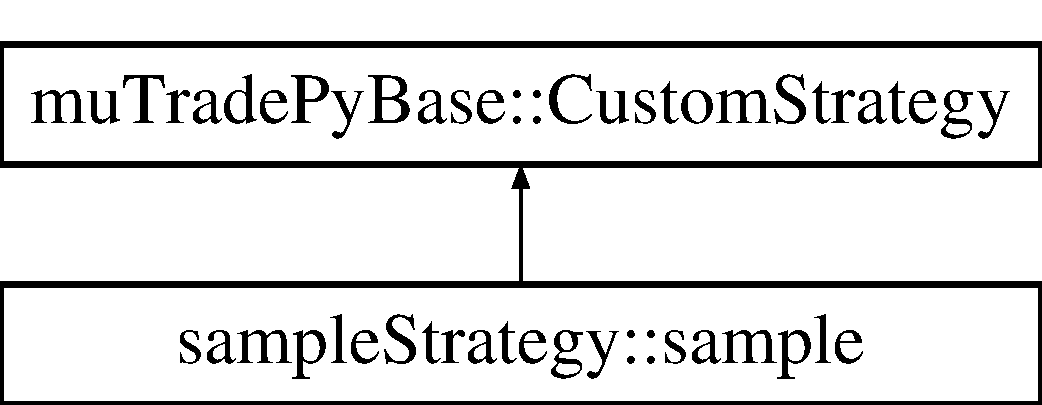
\includegraphics[height=2.000000cm]{classsampleStrategy_1_1sample}
\end{center}
\end{figure}
\subsection*{Public Member Functions}
\begin{DoxyCompactItemize}
\item 
\hypertarget{classsampleStrategy_1_1sample_a824adf637925f01e6e95a68695e0a8df}{def {\bfseries \-\_\-\-\_\-init\-\_\-\-\_\-}}\label{classsampleStrategy_1_1sample_a824adf637925f01e6e95a68695e0a8df}

\item 
\hypertarget{classsampleStrategy_1_1sample_a0276042f0a48f1b13bb24d7c5a980f6a}{def {\bfseries on\-Init\-Event}}\label{classsampleStrategy_1_1sample_a0276042f0a48f1b13bb24d7c5a980f6a}

\item 
\hypertarget{classsampleStrategy_1_1sample_ae189229b773474fc8b01e519a3d1a354}{def {\bfseries on\-C\-M\-D\-Modify\-Strategy}}\label{classsampleStrategy_1_1sample_ae189229b773474fc8b01e519a3d1a354}

\item 
\hypertarget{classsampleStrategy_1_1sample_a8772d8f9aecaf9e7fb9f9a0aa087435d}{def {\bfseries on\-C\-M\-D\-Terminate\-Startegy}}\label{classsampleStrategy_1_1sample_a8772d8f9aecaf9e7fb9f9a0aa087435d}

\item 
\hypertarget{classsampleStrategy_1_1sample_ad24fe84a685be8bf30434275ff46700c}{def {\bfseries on\-C\-M\-D\-Terminate\-Sq\-Off\-Strategy}}\label{classsampleStrategy_1_1sample_ad24fe84a685be8bf30434275ff46700c}

\item 
\hypertarget{classsampleStrategy_1_1sample_a837817933dcbaa2bcf6c6d79a7f99a0d}{def {\bfseries on\-Market\-Data\-Event}}\label{classsampleStrategy_1_1sample_a837817933dcbaa2bcf6c6d79a7f99a0d}

\item 
\hypertarget{classsampleStrategy_1_1sample_a2d63e2ced58bf5712c1e6f7e85cf5cf5}{def {\bfseries on\-Ohlc\-Time\-Out\-Event}}\label{classsampleStrategy_1_1sample_a2d63e2ced58bf5712c1e6f7e85cf5cf5}

\item 
\hypertarget{classsampleStrategy_1_1sample_a80d7ffc2501684bf05ffb5f436eb106b}{def {\bfseries on\-Confirmed}}\label{classsampleStrategy_1_1sample_a80d7ffc2501684bf05ffb5f436eb106b}

\item 
\hypertarget{classsampleStrategy_1_1sample_a40b6a062417472d03b4631b7a27916f4}{def {\bfseries on\-Replaced}}\label{classsampleStrategy_1_1sample_a40b6a062417472d03b4631b7a27916f4}

\item 
\hypertarget{classsampleStrategy_1_1sample_a1cc4858996ea43ac462f030b6720088e}{def {\bfseries on\-Replace\-Rejected}}\label{classsampleStrategy_1_1sample_a1cc4858996ea43ac462f030b6720088e}

\item 
\hypertarget{classsampleStrategy_1_1sample_aa3d18273289d513d6abe5fc04a67b751}{def {\bfseries on\-Cancel\-Rejected}}\label{classsampleStrategy_1_1sample_aa3d18273289d513d6abe5fc04a67b751}

\item 
\hypertarget{classsampleStrategy_1_1sample_adaccfc4c93c1246ba20206f37d2052c3}{def {\bfseries on\-New\-Rejected}}\label{classsampleStrategy_1_1sample_adaccfc4c93c1246ba20206f37d2052c3}

\item 
\hypertarget{classsampleStrategy_1_1sample_a488f5f86c3fb036432f01d6f6f37cb83}{def {\bfseries on\-I\-O\-C\-Cancelled}}\label{classsampleStrategy_1_1sample_a488f5f86c3fb036432f01d6f6f37cb83}

\item 
\hypertarget{classsampleStrategy_1_1sample_a7e4f23b6fa39aba0065c268913b98ef3}{def {\bfseries on\-Filled}}\label{classsampleStrategy_1_1sample_a7e4f23b6fa39aba0065c268913b98ef3}

\item 
\hypertarget{classsampleStrategy_1_1sample_a167412a5ffdc877b00ab0273eb773099}{def {\bfseries on\-Partial\-Fill}}\label{classsampleStrategy_1_1sample_a167412a5ffdc877b00ab0273eb773099}

\item 
\hypertarget{classsampleStrategy_1_1sample_a1f1606ccf7f97d7b969c7a00a5d95793}{def {\bfseries on\-Market\-To\-Limit}}\label{classsampleStrategy_1_1sample_a1f1606ccf7f97d7b969c7a00a5d95793}

\item 
\hypertarget{classsampleStrategy_1_1sample_a4337acef57f06773fdd1c5cc09d40441}{def {\bfseries on\-Frozen}}\label{classsampleStrategy_1_1sample_a4337acef57f06773fdd1c5cc09d40441}

\item 
\hypertarget{classsampleStrategy_1_1sample_a3a5c986bc3d0eb22af8fe51c02c37c22}{def {\bfseries on\-Timer\-Event}}\label{classsampleStrategy_1_1sample_a3a5c986bc3d0eb22af8fe51c02c37c22}

\end{DoxyCompactItemize}
\subsection*{Public Attributes}
\begin{DoxyCompactItemize}
\item 
\hypertarget{classsampleStrategy_1_1sample_a918c4c9d2bbf76d992818bbb9e560aa4}{{\bfseries f}}\label{classsampleStrategy_1_1sample_a918c4c9d2bbf76d992818bbb9e560aa4}

\item 
\hypertarget{classsampleStrategy_1_1sample_a6d2312273f20c1c5a07373b253e5e64d}{{\bfseries Trade\-Instrument}}\label{classsampleStrategy_1_1sample_a6d2312273f20c1c5a07373b253e5e64d}

\end{DoxyCompactItemize}


The documentation for this class was generated from the following file\-:\begin{DoxyCompactItemize}
\item 
sample\-Strategy.\-py\end{DoxyCompactItemize}

\chapter{File Documentation}
\hypertarget{muTradePyBase_8py}{
\section{muTradePyBase.py File Reference}
\label{muTradePyBase_8py}\index{muTradePyBase.py@{muTradePyBase.py}}
}
\subsection*{Classes}
\begin{DoxyCompactItemize}
\item 
class \hyperlink{classmuTradePyBase_1_1CustomStrategy}{muTradePyBase::CustomStrategy}
\end{DoxyCompactItemize}
\subsection*{Namespaces}
\begin{DoxyCompactItemize}
\item 
namespace \hyperlink{namespacemuTradePyBase}{muTradePyBase}
\end{DoxyCompactItemize}

\hypertarget{README_8md}{
\section{README.md File Reference}
\label{README_8md}\index{README.md@{README.md}}
}

\hypertarget{sampleStrategy_8py}{
\section{sampleStrategy.py File Reference}
\label{sampleStrategy_8py}\index{sampleStrategy.py@{sampleStrategy.py}}
}
\subsection*{Classes}
\begin{DoxyCompactItemize}
\item 
class \hyperlink{classsampleStrategy_1_1sample}{sampleStrategy::sample}
\end{DoxyCompactItemize}
\subsection*{Namespaces}
\begin{DoxyCompactItemize}
\item 
namespace \hyperlink{namespacesampleStrategy}{sampleStrategy}
\end{DoxyCompactItemize}

\printindex
\end{document}
